\documentclass[./main.tex]{subfiles}
\begin{document}

En el capítulo anterior estudiamos los regímenes dinámicos del modelo de fase con bifurcación de ciclo infinito y ruido blanco gaussiano aditivo. Observamos que, en su régimen excitable, este modelo presenta actividad pulsátil e intervalos de silencio. El ruido promueve la presencia de la actividad pulsátil que irrumpe en los silencios, y simultáneamente regula su coherencia. Analizamos que es posible obtener actividad pulsátil con cierta regularidad modulando los valores del ruido. Por otro lado, observamos que en el régimen oscilatorio del modelo, el ruido promueve la disminución de la coherencia de la actividad oscilatoria, es decir, desordena las oscilaciones. Estas características convierten a este modelo en un candidato interesante para describir las oscilaciones intermitentes, ya que podríamos interpretarlas como actividad pulsátil con cierta coherencia, u oscilaciones desordenadas. Comenzaremos por evaluar si con este modelo es posible reproducir la dinámica observada en los experimentos, o si es necesario proponer modificaciones al modelo para incorporar aspectos de la dinámica de actividad de ERK que el modelo no puede reproducir.


Primero nos preguntamos si las propiedades dinámicas de esta descripción teórica son compatibles con las observaciones experimentales. Para esto, comparamos simultáneamente la estadística de ciertos observables simples calculada sobre el modelo teórico con la de los datos experimentales. A partir de observar compatibilidad, diseñamos un protocolo para ajustar de manera sistemática los observables calculados sobre el modelo teórico a los calculados sobre los experimentos. Para valorar este ajuste, evaluamos si las principales características dinámicas que describen las oscilaciones intermitentes en nuestras observaciones experimentales -más complejas e informativas que los observables que ajustamos- pueden ser recapituladas por el modelo. Nuestros resultados sugieren que esta descripción falla en reproducir la heterogeneidad de actividad que observamos en los datos experimentales, y el modelo es insuficiente para describir las oscilaciones intermitentes de actividad de ERK en ESCs. 


Motivados por el análisis de estos resultados, proponemos modificaciones al modelo, y exploramos la idea de que la actividad pulsátil de ERK pueda ser descripta a partir de transiciones entre el régimen oscilatorio y el excitable, que sin perturbaciones dará lugar a intervalos de silencio. Transiciones breves darían lugar a pulsos aislados, y transiciones más largas a trenes de pulsos. Para esto, estudiamos los efectos de proponer fluctuaciones lentas en la amplitud de modulación del modelo de fase con bifurcación de ciclo infinito. A partir de implementar un nuevo ajuste, encontramos que el modelo falla en reproducir la estadística de pulsos aislados que observamos en los experimentos. Como alternativa, analizamos si es posible describir la dinámica de actividad de ERK como un sistema dinámico que simultáneamente de lugar a transiciones entre los regímenes dinámicos oscilatorio y excitable, y tenga perturbaciones capaces de generar actividad pulsátil en el excitable, y de esta manera generar pulsos aislados. Encontramos que con esta descripción es posible recapitular las principales características dinámicas que describen las oscilaciones intermitentes en nuestras observaciones experimentales. En el resultado del ajuste, las fluctuaciones tienen escalas temporales lentas en comparación con la duración de las series temporales que buscamos reproducir. Para finalizar, evaluamos si las fluctuaciones que representamos en la amplitud de modulación pueden ser incorporadas como procesos estacionarios, y no como un proceso que varíe durante cada medición como hipotetizamos en los dos casos anteriores. 

\section{El modelo de fase con bifurcación de ciclo infinito con ruido blanco gaussiano no logra reproducir la actividad pulsátil heterogénea}
\sectionmark{El modelo de fase con ruido blanco ...}
\label{C6_sec:alder_ruido_fit}

En esta sección evaluamos si perturbando de manera sistemática al sistema en el régimen excitable o mediante oscilaciones desordenadas es posible reproducir las principales características dinámicas de las oscilaciones intermitentes, ya sean interpretándolas como actividad pulsátil con cierta coherencia, o como oscilaciones desordenadas. En simultáneo, presentamos las herramientas técnicas y la metodología para comparar experimentos con teoría que utilizaremos en el resto del capítulo. Primero proponemos observables simples para comparar la estadística del modelo teórico con la de los datos experimentales. Luego, introducimos una estrategia para detectar pulsos y adquirir mediciones de estos observables sobre series temporales simuladas. A continuación, evaluamos si la estadística de estos observables es compatible con las mediciones de actividad dinámica de ERK realizadas en el capítulo \ref{ch2}. Finalmente, introducimos un método para ajustar los observables calculados sobre el modelo teórico a los calculados sobre los experimentos, y evaluamos si los resultados del ajuste reproducen las principales características dinámicas que describen las oscilaciones intermitentes comparando simulaciones numéricas con los principales resultados de la caracterización de la dinámica de activación de ERK que obtuvimos en ese capítulo. 



\subsection{Observables para comparar la teoría con los experimentos}

Para comparar el modelo con los datos experimentales, decidimos enfocarnos en la estadística de la duración de pulsos (ecuación \ref{C2_eq:duracion_de_pulsos}, figura \ref{C6_fig:observables_experimentales}A), el intervalo de interpulsado (ecuación \ref{C2_eq:IPI}, figura \ref{C6_fig:observables_experimentales}B), y la tasa de pulsado -definida como el número de pulsos dividido por la duración de la serie temporal- (sección \ref{C3_ssec:analisis_cuantitativo}, figura \ref{C6_fig:observables_experimentales}C). Elegimos la duración de pulsos porque consideramos que es una característica clave que describe dinámica de los pulsos individuales. El intervalo de interpulsado es una medida cuantitativa simple que informa acerca de cómo están ordenados los pulsos en la serie temporal. Finalmente, la tasa de pulsado es una medida sencilla de la actividad pulsátil en las series temporales experimentales. Esperamos, además, que el ajuste simultáneo de la duración de pulsos y la tasa de pulsado conduzca a ajustar el tiempo medio que las células estuvieron pulsando (ecuación \ref{C2_eq:actividad}, figura \ref{C2_fig:actividad}). Para comparar el modelo con los experimentos, calculamos la estadística de estos observables en el modelo teórico midiendo estas cantidades en series temporales de la variable angular \xx en función del tiempo $t$, en donde las series temporales las obtenemos a partir de simulaciones numéricas (apéndice \ref{C6_ap:traces}).

\begin{figure}
    \centering
    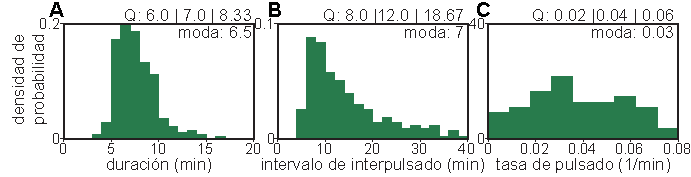
\includegraphics[width=1\columnwidth]{figures/chapter6/C6_experimental_stats.pdf} 
    \caption{\textbf{Observables representativos de los datos experimentales.} (A) Distribución de la duración de pulsos. Las unidades del eje $y$ son 1/min. (B) Distribución de intervalo de interpulsado. Las unidades del eje $y$ son 1/min. (C) Distribución de tasa de pulsado. Las unidades del eje $y$ son min. (A-C) Los datos experimentales fueron adquiridos en serum + LIF (capítulo \ref{ch2}). N = 69 células, $n_1$ = 289 pulsos, $n_2$ = 225 pares de pulsos. Los cuartiles (Q) 25, 50 y 75 y la moda se indican en la parte superior de cada gráfico. Fueron excluidos de los histogramas 9 (en B) y 7 (en C) puntos mayores que el límite del eje $x$.}
    \label{C6_fig:observables_experimentales}
\end{figure}


Retomando las definiciones de la sección \ref{C6_sec:duracion}, definimos un pulso en el régimen excitable del modelo de fase con bifurcación de ciclo infinito y ruido blanco gaussiano aditivo de la ecuación \ref{C6_eq:adler_white_noise} cuando el sistema sobrepasa el punto fijo inestable \xxi y realiza una excursión hacia el punto fijo estable siguiente \xxe sin volver a \xxi. En estas circunstancias, en las series temporales de la fase el inicio del pulso es el punto fijo inestable \xxi, y su final es el punto fijo estable siguiente \xxe. Para el caso oscilatorio, definimos un pulso cuando el sistema alcanza $\xx_0+2\pi$, habiendo partido y no vuelto a $\xx_0$.  Es decir, el inicio del pulso es un punto arbitrario $\xx_0$, y el final del pulso es $\xx_0+2\pi$. Con estas definiciones en mente, la \textbf{duración de pulsos}\marginpar{duración de pulsos} es el tiempo que transcurre entre el inicio y el final de cada pulso. En el régimen oscilatorio elegiremos $\xx_0 = -\pi/2 + 2n\pi$, el punto de la circunferencia donde aparece la bifurcación (figuras \ref{C5_fig:adler_determinista_oscilatorio},\ref{C5_fig:adler_determinista_excitable}). \marginpar{intervalo de\\interpulsado}Definimos el \textbf{intervalo de interpulsado} como el tiempo que tarda el sistema en ir desde $\xx_i = 3\pi/2+ 2n\pi$ hacia $\xx_f = 3\pi/2 + 2(n+1)\pi$, aunque podríamos haber implementado esta definición en cualquiera de los puntos de la circunferencia que tenga una distancia angular de $2\pi$. En el oscilatorio, esta definición es análoga a la duración de pulsos, lo que es una característica de sistemas oscilatorios.\marginpar{tasa de pulsado} Por último, definimos la \textbf{tasa de pulsado} como el número de pulsos divido la duración de la serie temporal.  

\subsection{Medición de los observables en el modelo teórico}
\label{C6_ssec:deteccion_de_pulsos}

Para medir la duración de pulsos y la tasa de pulsado en series temporales de la variable angular \xx en función del tiempo $t$, desarrollamos un algoritmo de detección de pulsos. En esta detección, requerimos identificar los mínimos que determinan el comienzo y el final de un pulso. Con esta información, podremos también comparar el modelo con los experimentos mediante el análisis realizado en el capítulo \ref{ch2}. A continuación, describimos brevemente el algoritmo, y visualizaremos los pasos intermedios en el observable \ref{C5_eq:seno_fase}, pues es más simple ver pulsos en el observable que en la serie temporal de la fase en función del tiempo (figura \ref{C6_fig:pulse_detection}A). Nos enfocaremos en describir el algoritmo para el caso excitable, y su extensión al caso oscilatorio es casi inmediata.


Primero buscamos establecer puntos de referencia a partir de donde buscaremos el comienzo y el final de cada pulso. Comenzamos por identificar los máximos y mínimos locales de la serie temporal $X = \sin{\theta}$, imponiendo dos condiciones: (i) que los máximos (o mínimos) sean mayores (o menores) que un umbral de amplitud $A_{\text{th}}$ (o $-A_{\text{th}}$), y (ii) que los máximos (o mínimos) consecutivos estén separados por al menos una distancia umbral $W_{\text{th}}$. 


Para detectar cada máximo local, recorreremos la serie temporal $X$ en la dirección del tiempo, evaluando cada $X_j$ en la dirección en la que crece el índice temporal $j$, donde $W_{\text{th}} < j \leq N - W_{\text{th}}$ y $N$ es la longitud de la serie temporal $X$. Por simplicidad, decidimos no incluir los bordes de $X$ en el análisis. Para cada $X_j$, si $X_j > A_{\text{th}}$ resultará un candidato a máximo local. Este procedimiento resulta en un subconjunto de candidatos a máximos locales que sobrepasan el umbral de amplitud. Dentro de este subconjunto, retenemos sólo aquellos candidatos que sean mayores o iguales a sus máximos vecinos del intervalo $\left[ X_{j-W_{\text{th}}},X_{j+W_{\text{th}}}\right]$. En caso de haber dos o más candidatos a máximos locales iguales dentro de dicho intervalo, conservamos uno elegido al azar. Realizamos un procedimiento análogo para determinar los mínimos locales. El resultado de este paso intermedio se encuentra representado en la figura \ref{C6_fig:pulse_detection}B.
 
 
 \begin{figure}
    \centering
    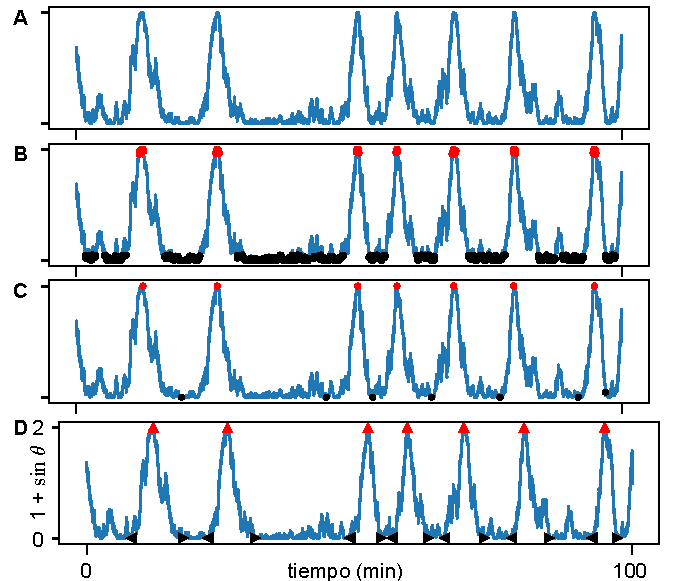
\includegraphics[width=1\columnwidth]{figures/chapter6/C6_pulse_detection.pdf} 
    \caption{\textbf{Algoritmo de detección de pulsos para calcular la duración de pulsos y la tasa de pulsado.} (A) Serie temporal adquirida en simulaciones numéricas (apéndice \ref{C6_ap:traces}). (B) Paso intermedio del algoritmo de detección de pulsos, donde los máximos (rojo) y mínimos (negro) relativos que cumplen las condiciones umbrales están indicados. (C)  Paso intermedio del algoritmo de detección de pulsos, donde los máximos M (rojo) y mínimos m (negro) de referencia obtenidos luego del filtrado están indicados. (D) Resultado del algoritmo de detección de pulsos, donde el inicio (triángulo negro con el vértice del lado izquierdo), el pico (rojo) y el final (triángulo negro con el vértice del lado derecho) están indicados. Parámetros: $\omega = 2\pi/ 7 \; \text{min}^{-1}$, $\alpha = 1.01 \times  2\pi/ 7 \; \text{min}^{-1}$, $ D = 0.1 \; \text{min}^{-2}$. La tasa de adquisición fue de dt = 0.001, cada d = 1 pasos. El umbral de amplitud del algoritmo de detección de pulsos fue $A_{\text{th}} = 0.9$, y la distancia umbral fue $W_{\text{th}} = 100\text{ cuadros}$.} 
    \label{C6_fig:pulse_detection}
\end{figure}
 

Continuamos por imponer que entre dos máximos locales haya un sólo mínimo, y que entre dos mínimos locales haya un máximo. Primero removemos todos los mínimos locales detectados antes del primer máximo local. Luego recorremos todos los pares de máximos locales sucesivos que detectamos. Empezamos por el primero y el segundo, continuamos por el segundo y el tercero, y así sucesivamente. Para cada par de máximos locales consecutivos, tomamos todos los mínimos locales que hayamos detectado entre ellos. Luego, removemos, de a uno, el mayor de este subgrupo de mínimos locales detectados, hasta tener un solo mínimo local. Si este subgrupo estaba inicialmente vacío, removemos el máximo menor del par de máximos locales que consideramos, y comenzamos otra vez redefiniendo el par de máximos sucesivos. Una vez recorridos todos los pares de máximos locales, removemos todos los mínimos detectados después del último máximo, a excepción del primero. Con este procedimiento, logramos tener la misma cantidad de máximos y mínimos locales. Los máximos y mínimos locales funcionan como puntos de referencia a partir de donde buscaremos el comienzo y el final de cada pulso. A los máximos de referencia los llamaremos $M$, y a los mínimos de referencia $m$. La cantidad de los máximos de referencia $M$ es la misma que la de los mínimos de referencia $m$. Entonces, decimos que cada máximo $M_k$ tiene asociado un mínimo de referencia inmediatamente anterior $m_{k-1}$, y uno inmediatamente posterior $m_{k}$, a excepción del primer máximo $M_0$. El resultado de este paso intermedio se encuentra representado en la figura \ref{C6_fig:pulse_detection}C.


Los máximos de referencia $M$ se corresponden con un máximo en $\sin{\xx}$, es decir, en $\xx \approx \pi/2 + 2n\pi$. Los mínimos de referencia $m$ se corresponden con un mínimo en $X\sin{\xx}$, es decir, en $\xx \approx 3\pi/2 + 2n\pi$. Entonces, si nos paramos sobre un máximo $M_k$ y recorremos la fase en dirección contraria al tiempo hacia su mínimo inmediatamente anterior $m_{k-1}$, atravesaremos un punto fijo inestable. En cambio, si nos paramos sobre un máximo $M_k$ y recorremos la fase en la dirección del tiempo hacia su mínimo inmediatamente posterior $m_{k}$, atravesaremos el punto fijo estable (figura \ref{C5_fig:adler_determinista_excitable}). Con esta idea buscaremos el principio y el final de los pulsos. Para cada máximo de referencia $M_k$, calculamos su número de vueltas completas $n$ que tiene la fase en ese instante, y se lo restamos momentáneamente a la variable angular $\xx' = \xx - 2n \pi$. Con esta transformación, $M_k$ queda posicionado entre el primer y segundo cuadrante, $m_{k-1}$ entre los cuadrantes $-1$ y $-2$, y $m_{k+1}$ entre los cuadrantes $3$ y $4$. Además, \xxe queda posicionado en el cuadrante $-1$, y \xxi en el cuadrante $3$. Recorremos la fase $\xx'$ desde el máximo $M_k$ en dirección contraria al tiempo hacia el mínimo inmediatamente anterior $m_{k-1}$. En esta dirección, esperamos que la fase \xx en promedio decrezca. En el caso del primer máximo, el final del recorrido es comienzo de la serie temporal. Cuando $\xx' - \xxe' \geq 0$, encontramos el punto fijo estable $C_k$, que consideramos el comienzo de un pulso. Puede ocurrir que no nos topemos con un punto fijo estable durante este recorrido. Por ejemplo, puede suceder con altos valores de ruido la fase decrezca con el tiempo y no atraviese un punto fijo inestable. Como interpretamos ciclos de la fase como pulsos de ERK, en estos casos descartamos $M_k$ y su mínimo inmediatamente posterior $m_k$. Otro ejemplo es que en el caso oscilatorio puede que no encontremos al comienzo del pulso durante este recorrido, pues esperamos que el comienzo del pulso tenga una fase muy parecida al mínimo $m_{k-1}$. En ese caso, continuamos recorriendo la fase hasta el máximo $M_{k-1}$ inmediatamente anterior a $M_k$. En caso de no encontrar el punto fijo durante este recorrido, descartamos $M_k$ y su mínimo inmediatamente posterior $m_k$. Realizamos un procedimiento análogo para encontrar el punto fijo inestable $F_k$, es decir, el final de cada pulso, en este caso recorriendo la fase $\xx'$ desde $M_k$ hacia su mínimo inmediatamente posterior $m_k$. Como resultado de este procedimiento, tendremos un conjunto de puntos fijos inestables $C$ que marcan el comienzo de los pulsos, un conjunto de máximos $M$ que señalizan el pico de un pulso, y un conjunto de puntos fijos estables $F$ que representan el final de los pulsos (figura \ref{C6_fig:pulse_detection}D). Con estos resultados, calculamos la duración de cada pulso $k$ como el tiempo que transcurre entre el principio $C_k$ y el final $F_k$ del pulso, y la tasa de pulsado como la cantidad de pulsos detectados en cada serie temporal $l$ sobre la duración de la serie temporal $T_l$. 


Para calcular el intervalo de interpulsado, recorremos la serie temporal desde su inicio en dirección del tiempo. Para inicializar el procedimiento, anotamos el primer punto $Y_i$ cuya diferencia entre su fase y $3\pi/2$ sea mayor o igual que $2\pi$. Luego, continuado el recorrido, buscamos el primer punto $Y_f$ tal que la diferencia de fases entre $Y_f$ e $Y_i$ sea mayor o igual a $2\pi$. Una vez encontrado $Y_1$, el tiempo que transcurre entre $Y_f$ e $Y_i$ va a ser la primera medición de intervalo de interpulsado. Luego, repetimos el procedimiento  con $Y_f \rightarrow Y_i$ hasta terminar la serie temporal. Las mediciones realizadas con este método mostraban una estadística muy similar, pero un poco menos ruidosa, a calcular el intervalo de interpulsado como la diferencia temporal entre los picos de dos pulsos sucesivos $M_k$ y $M_{k+1}$ identificados a partir del algoritmo de detección de pulsos. Por esto optamos por medir el intervalo de interpulsado con esta estrategia. 


\subsection{Evaluación de la compatibilidad de la teoría con los experimentos}

Para evaluar si las propiedades dinámicas de la descripción teórica son compatibles con las observaciones experimentales, primero observamos cómo dependen la duración de pulsos, el intervalo de interpulsado y la tasa de pulsado de los parámetros del modelo. Luego, evaluamos si existe alguna región de parámetros en donde la estadística de los tres observables calculados sobre datos simulados sea compatible con nuestras observaciones sobre los datos experimentales simultáneamente. 

Para esto, obtuvimos series temporales de la fase a partir de simulaciones (apéndice \ref{C6_ap:traces}). A partir de estas series temporales, calculamos las distribuciones de la duración de pulsos, el intervalo de interpulsado y la tasa de pulsado. Para observar el comportamiento de estos observables cuando varían los parámetros del modelo, nos enfocamos en un estadístico simple como es la mediana de las distribuciones. De esta forma, podíamos visualizar más fácilmente la dependencia de los observables de lo parámetros del modelo mediante grillas bidimensionales. Exploramos la mediana de la distribución de duración de pulsos en una grilla bidimensional de parámetros (figura \ref{C6_fig:2d_plots}A). Para interpretar este gráfico, es útil enfocarse en el caso determinista representado por la línea vertical $D=0$, donde sólo varía la amplitud de modulación. En este caso, los valores de la amplitud de modulación menores que la frecuencia del uniforme darán lugar al régimen oscilatorio (sector inferior a la linea punteada negra), y valores de la amplitud de modulación mayores que la frecuencia del uniforme darán lugar al régimen excitable (sector superior a la linea punteada negra). Por ejemplo, cuando $\omega = 2\pi/7\; \text{min}^{-1}$, observamos que a medida que aumenta la amplitud de modulación desde cero hasta el valor de $\omega$ , la duración de pulsos aumenta. Esto es coherente con nuestra caracterización previa, donde observamos que los aumentos en la amplitud de modulación en el modelo determinista conducen a oscilaciones no uniformes, y a medida que las oscilaciones son cada vez menos uniformes aumenta la duración de pulsos (sección \ref{C5_sec:osc_exc}, figura \ref{C5_fig:T_osc}). Cuando $\alpha$ supera el valor de $\omega$, no se detectan pulsos en el régimen excitable, pues $D=0$ y no hay perturbaciones que puedan desencadenar actividad pulsátil. Si, en cambio, nos enfocamos en la línea horizontal donde $\alpha=0$, estaremos evaluando el caso de oscilaciones uniformes con ruido blanco gaussiano aditivo. Vemos en este caso que la duración de pulsos disminuye de izquierda a derecha conforme aumenta y domina el ruido por sobre el sistema dinámico (sección \ref{C6_sec:alder_ruido},figura \ref{C6_fig:duration}). Con este enfoque, observamos en la figura \ref{C6_fig:2d_plots}A que, para una dada frecuencia del uniforme, en el régimen oscilatorio la duración de pulsos disminuye en sentido diagonal desde arriba a la izquierda hacia abajo a la derecha, es decir, cuando aumenta la intensidad del ruido y disminuye la amplitud de modulación simultáneamente. Además, para valores de ruido pequeños menores a $0.4 \;\text{min}^{-2}$, parece haber un cambio en el comportamiento de la duración de pulsos en función de la amplitud de modulación cuando se reduce la frecuencia del uniforme. Por otro lado, en el régimen excitable la duración de pulsos disminuye desde abajo a la izquierda hacia arriba a la derecha, conforme aumentan la amplitud de modulación y la intensidad del ruido, en sentido diagonal opuesto al caso oscilatorio. Esta diferencia de comportamientos se ve acompañada por una discontinuidad o diferencia pronunciada en $\dddelta = 1$, donde se produce la bifurcación. Además, los valores de la duración de pulsos disminuyen conforme aumenta la frecuencia del uniforme. Todas estas observaciones son consistentes con nuestros resultados analíticos previos (sección \ref{C6_sec:duracion}, figura \ref{C6_fig:duration}).

 \begin{figure}
    \centering 
    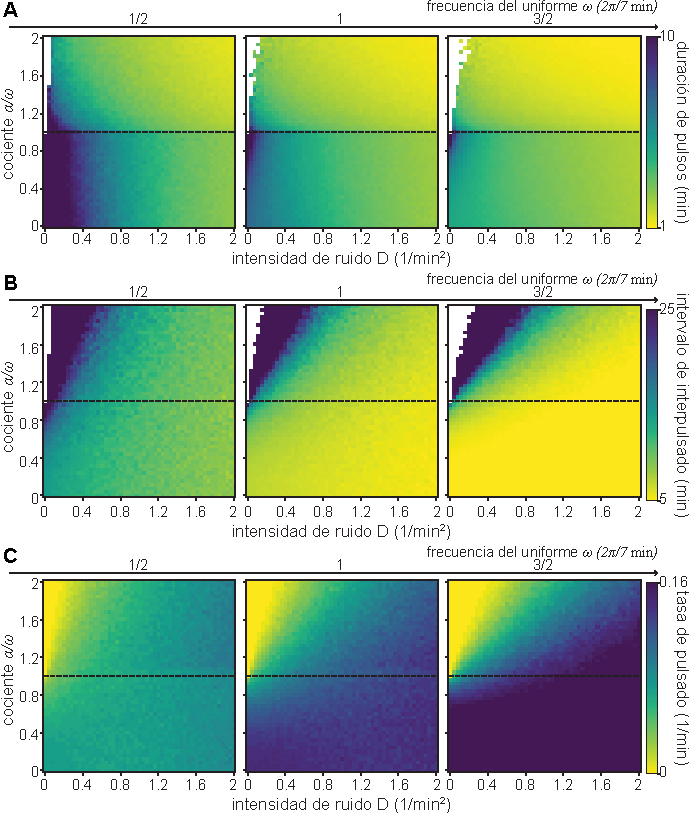
\includegraphics[width=1\columnwidth]{figures/chapter6/C6_2d_plots.pdf} 
    \caption{\textbf{Comportamiento de los observables elegidos en función de los parámetros del modelo}. Mediciones numéricas de la mediana de (A) la duración de pulsos, (B) el intervalo de interpulsado y (C) la tasa de pulsado en función de los parámetros del modelo. (A-C) Se observa el comportamiento en función de la intensidad del ruido $D$  y la amplitud de modulación $\alpha$ normalizada por la frecuencia del uniforme $\omega$. En cada caso, la frecuencia del uniforme es fija y su valor está indicado en la parte superior de cada gráfico. Los sectores blancos indican regiones donde no había actividad pulsátil en los datos simulados. La linea punteada negra indica el punto de bifurcación que separa el régimen oscilatorio (abajo) del excitable (arriba). La resolución del cociente \dddelta es $0.04\; \text{min}^{-1}$, y de la intensidad de ruido es $0.04\; \text{min}^{-2}$. Cada punto de cada gráfico representa la adquisición del observable correspondiente sobre una serie temporal de $T = 10000$ minutos de duración. La tasa de adquisición fue de $dt = 0.0001$, cada $d = 10$ pasos. El umbral de amplitud del algoritmo de detección de pulsos fue $A_{\text{th}} = 0.9$, y la distancia umbral fue de $W_{\text{th}} = 100 $ cuadros.}
    \label{C6_fig:2d_plots}
\end{figure}


La mediana de la distribución de intervalo de interpulsado medida sobre las series temporales simuladas de la fase se encuentra representada en la figura \ref{C6_fig:2d_plots}B. Para una misma frecuencia del uniforme, este observable disminuye conforme aumenta la intensidad del ruido y disminuye la amplitud de modulación en ambos regímenes dinámicos. A diferencia de la duración de pulsos, en este caso no parece haber una discontinuidad o diferencia pronunciada de comportamiento en la transición entre los regímenes dinámicos oscilatorio y excitable. Los valores de intervalo de interpulsado disminuyen conforme aumenta la frecuencia del uniforme. En la figura \ref{C6_fig:2d_plots}C observamos que la tasa de pulsado presenta un comportamiento opuesto a la distribución de intervalos de interpulsado. En este caso, la tasa de pulsado aumenta conforme aumenta la intensidad del ruido, disminuye la amplitud de modulación tanto en el régimen excitable como en el oscilatorio, y sus valores aumentan con la frecuencia del uniforme. Aunque sean opuestos, los comportamientos de ambos observables tienen origen en que la actividad pulsátil aumenta en esa dirección. Este aumento de actividad resulta en intervalos de interpulsado más cortos y tasas de pulsado más grandes. 


Para estudiar la compatibilidad de estas tres medidas con los valores adquiridos experimentalmente, identificamos en qué regiones de los mapas bidimensionales los valores de las medianas de cada observable estaban incluidos dentro de los rangos intercuartílicos de las distribuciones experimentales de la figura \ref{C6_fig:observables_experimentales}. En la figura \ref{C6_fig:2d_plots_sup}A coloreamos en negro los valores de la mediana de la duración de pulsos, el intervalo de interpulsado y la tasa de pulsado medidas en simulaciones si éstos se encontraban en el intervalo definido entre el primer (Q25) y tercer cuartil (Q75) de las correspondientes distribuciones experimentales.


Para todos los casos vemos que el área de la zona de coincidencia disminuye conforme aumenta la frecuencia del uniforme. Recordemos que los valores modales de la duración de pulsos y el intervalo de interpulsado de los experimentos eran alrededor de 7 minutos (figura \ref{C6_fig:observables_experimentales}). Que la zona de coincidencia de la duración de pulsos esté mayoritariamente ubicada en el régimen oscilatorio y en regiones de ruido pequeño para $\omega = 2\pi/7 \text{min}^{-1}$ posiblemente refleje esta característica, puesto que en las oscilaciones uniformes la duración de pulsos es en promedio 7 minutos. Que la zona de coincidencia se traslade a regiones de ruido mayores para frecuencias del uniforme más pequeñas para reproducir los valores de duración de pulsos que observamos en los experimentos es consistente con que la duración de pulsos disminuye en esa dirección. Además, que la región de coincidencia en el régimen oscilatorio sea casi rectangular para los valores intermedio y pequeño de frecuencia del uniforme que consideramos es producto de la pendiente pequeña que tiene la duración de pulsos en función de la amplitud de modulación, fenómenos que observamos en el resultado analítico para esos valores (figura \ref{C6_fig:duration}C,D). Por otro lado, el rango intercuartílico del intervalo de interpulsado posee información sobre cómo están ordenados los pulsos, y el de la tasa de pulsado sobre la cantidad de pulsos. Que el área de sus zonas de coincidencia aumente para valores más pequeños de frecuencias del uniforme que $\omega = 2\pi/7 \text{min}^{-1}$ posiblemente tenga origen en la diferencia entre oscilaciones uniformes, donde hay un pulso por lo general detrás del otro, y las oscilaciones intermitentes de actividad de ERK que observamos en los experimentos, donde hay pulsos que son aislados y están alejados de sus pulsos vecinos.  

Buscamos delimitar regiones de parámetros compatibles con los experimentos donde había superposición en los tres observables simultáneamente. En la figura \ref{C6_fig:2d_plots_sup}B observamos que existen regiones de parámetros en donde la estadística del modelo ajusta a las observaciones experimentales. En todos los casos, las regiones de compatibilidad se encontraban cerca de la zona de bifurcación. Además, vimos que estas zonas aumentan su área conforme se reduce la frecuencia del oscilatorio. Es posible que si continuamos reduciendo $\omega$, encontremos regiones más extensas de parámetros en donde el modelo es compatible con el experimento. En definitiva, este procedimiento nos informa que existen regiones del espacio de parámetros del modelo teórico considerado que reproducen los estadísticos medidos sobre los experimentos. Sin embargo, el enfoque es poco práctico para conseguir un ajuste de estos parámetros. Motivados por estos resultados, decidimos establecer un protocolo para ajustar de manera sistemática los parámetros del modelo, que describimos a continuación. 



 \begin{figure}
    \centering
    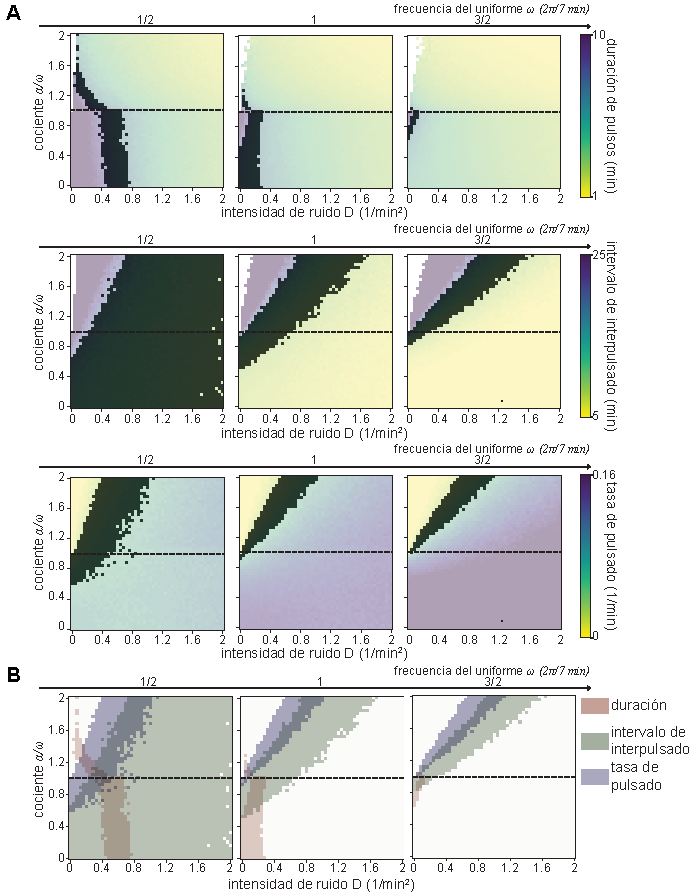
\includegraphics[width=1\columnwidth]{figures/chapter6/C6_2d_plots_superposition.pdf} 
    \caption{\textbf{Regiones de compatibilidad de los observables elegidos entre la teoría y los experimentos}. (A) Mediciones numéricas de la mediana de la duración de pulsos, el intervalo de interpulsado y la tasa de pulsado en función de los parámetros del modelo. En cada gráfico, se observa el comportamiento en función de la intensidad del ruido $D$ y la amplitud de modulación $\alpha$ normalizada por la frecuencia del uniforme $\omega$. En cada caso, la frecuencia del uniforme es fija y su valor está indicado en la parte superior. Los sectores negros indican las regiones donde los valores de las medianas adquiridas en el modelo teórico se encuentran dentro del rango intercuartilico de cada observable, definido como el intervalo entre el primer (Q25) y tercer (Q75) cuartil. Los sectores blancos indican regiones donde no había actividad pulsátil en los datos simulados. Cada punto de cada gráfico representa la adquisición del observable correspondiente sobre una serie temporal de $T = 10000$ minutos de duración. La tasa de adquisición fue de $dt = 0.0001$, cada $d = 10$ pasos. El umbral de amplitud del algoritmo de detección de pulsos fue $A_{\text{th}} = 0.9$, y la distancia umbral fue $W_{\text{th}} = 100\text{ cuadros}$. (B) Superposición de las regiones coloreadas en negro en A. En este caso, el sector blanco indica ausencia de superposición entre algún observable del modelo teórico y el experimento. (A,B) La linea punteada negra marca el punto de bifurcación que separa el régimen oscilatorio (abajo) del excitable (arriba). La resolución del cociente \dddelta es $0.04\; \text{min}^{-1}$, y de la intensidad de ruido es $0.04\; \text{min}^{-2}$.}
    \label{C6_fig:2d_plots_sup}
\end{figure}




\subsection{Implementación del Cálculo Bayesiano Aproximado Monte Carlo Secuencial para ajustar el modelo a los experimentos}
\subsectionmark{Implementación del ABC-SMC para ajustar el modelo a los experimentos}
%\subsection{Ajuste de las medidas experimentales}
\label{C6_sssec:implementac_ABCSMC}

Buscamos establecer un protocolo para ajustar de manera sistemática la estadística de duración de pulsos, intervalo de interpulsado y tasa de pulsado del modelo a la observada en las mediciones experimentales de la dinámica de actividad de ERK en ESCs (figura \ref{C6_fig:observables_experimentales}). Implementamos el método de Cálculo Bayesiano Aproximado (ABC, por \textit{Approximate Bayesian Computation}) basado en la implementación de Monte Carlo Secuencial (SMC, por \textit{Sequential Monte Carlo}) para obtener una distribución de probabilidad de los posibles $(\omega,\dddelta,D)$ que ajusten a nuestros datos experimentales.


%\subsubsection{Implementación del Cálculo Bayesiano Aproximado Monte Carlo Secuencial}
%\subsubsectionmark{Implementación del ABC-SMC}


%qué es el ABCMC
El método ABC-SMC busca inferir una distribución de probabilidad \textit{posterior} conjunta para los parámetros del modelo $(\omega,\dddelta,D)$, dada una distribución de probabilidad \textit{prior} que elegimos previamente para cada uno de los parámetros individuales \cite{Toni2009}.\marginpar{Cálculo Bayesiano\\Aproximado Monte\\Carlo Secuencial} Como punto de partida, definimos la \textit{prior} a partir de nuestro conocimiento previo del modelo en función de qué parámetros consideramos razonables para describir los datos experimentales. La \textit{posterior} nos dirá cuál es la probabilidad de que nuestros datos provengan de un dado grupo de parámetros $(\omega,\dddelta,D)$, dadas las mediciones experimentales.


% por qué elejimos el ABCMC
Por lo general, los métodos estadísticos bayesianos buscan obtener la \textit{posterior} a partir de la función de verosimilitud, una función de los parámetros del modelo teórico que es normalmente compleja o desconocida. La ventaja del método ABC es que evita evaluar las funciones de verosimilitud y utiliza, en su lugar, métricas que se calculan a partir de simulaciones numéricas \cite{Csillery2010}. Por otro lado, SMC es una técnica paralelizable y particularmente eficiente para recorrer el espacio de parámetros durante la implementación del ABC. Está demostrado que el método ABC-SMC bien diseñado converge a la distribución \textit{posterior}, independientemente de su inicialización \cite{Csillery2010,Filippi2013}. Aquí utilizamos la implementación de pyABC, disponible para python \cite{Klinger2018}.


%cómo lo implementamos 
Previo a la inicialización, definimos las \textit{prior} de cada uno de los parámetros $\omega,\dddelta,D$ como distribuciones uniformes dentro de intervalos que consideramos razonables luego de una inspección manual previa \cite{Toni2010} (ver apéndice \ref{C6_ap:ABC-SMC}). Para inicializar el método, se simulan una serie de series temporales a partir de $1000$ puntos $(\omega,\dddelta,D)$ muestreados del espacio tridimensional de parámetros definido por las \textit{prior}. Se calcula la distancia $d$ de cada serie temporal simulada con los datos experimentales (introduciremos y discutiremos la definición de distancia más adelante). En nuestra implementación, la mediana de estas distancias define la tolerancia $\epsilon$ que tendrá la primera iteración del algoritmo, y el peso (o probabilidad estimada) de cada uno de las mil muestras del espacio de parámetros es inicialmente $w = 1/1000$. 


En cada iteración, se elige un grupo de parámetros $(\omega,\dddelta,D)$ de los $1000$ aceptados previamente. Esta elección se realiza en función de los pesos $w$ asociados a cada uno de los puntos del espacio tridimensional aceptados en la iteración previa. Luego, se perturba el punto elegido buscando obtener uno nuevo \cite{Toni2009}. La manera en que se realiza esta perturbación influye en la eficiencia del algoritmo, pero no en su convergencia \cite{Filippi2013}. Nosotros elegimos realizarla con un \textit{kernel} gaussiano multivariado, y perturbamos cada grupo de parámetros aceptados según una distribución normal multivariada con una matriz de covarianza que depende de la covarianza de la población aceptada anteriormente. A partir del nuevo grupo de parámetros que surge de esta perturbación, se simula una serie temporal larga y se calcula su distancia $d$ a los datos experimentales (ver apéndice \ref{C6_ap:ABC-SMC}). Este nuevo grupo de parámetros será aceptado si la distancia entre los datos simulados y los experimentales es menor la tolerancia $\epsilon$ (figura \ref{C6_fig:eps}). Estas iteraciones se realizan hasta lograr aceptar nuevos $1000$ puntos del espacio tridimensional de parámetros. Una vez aceptados los nuevos $1000$ puntos, se actualiza las distribución de probabilidad conjunta de los parámetros y la tolerancia $\epsilon$. La distribución se actualiza calculando nuevos pesos $w$ de los grupos de parámetros aceptados, y aquí también utilizamos el \textit{kernel} gaussiano multivariado \cite{Toni2009}. Elegimos calcular la nueva tolerancia $\epsilon$ como la mediana de las distancias de la última población de grupos de parámetros aceptada. 

\begin{figure}
    \centering
    
\includegraphics[width=1\columnwidth]{figures/chapter6/C6_eps.pdf} 
    \caption{\textbf{Convergencia del Cálculo Bayesiano Aproximado Monte Carlo Secuencial.} Evolución de la tolerancia a medida que aumentan las iteraciones.}
    \label{C6_fig:eps}
\end{figure} 


Evaluamos la convergencia del método siguiendo el valor de la tolerancia, y establecimos una tolerancia mínima que determinaba el final del algoritmo \cite{Costa2021} (figura \ref{C6_fig:eps}, ver apéndice \ref{C6_ap:ABC-SMC}). El valor de la tolerancia mínima refleja la tensión entre el costo computacional y la precisión del método. Si la tolerancia mínima es suficientemente chica, la distribución \textit{posterior} obtenida será una buena aproximación de la real \cite{Toni2010}. El resultado es una muestra de $1000$ valores de parámetros a partir de la cual se infiere su distribución \textit{posterior} a través de sus pesos $w$ (ver apéndice \ref{C6_ap:ABC-SMC}). En definitiva, utilizamos una muestra finita de datos para hacer inferencias sobre la función de densidad de probabilidad subyacente en todo el espacio tridimensional de parámetros. Los \textit{kernels} gaussianos multivariados que utilizamos para realizar esta inferencia son una técnica no paramétrica para estimar estas funciones de densidad de probabilidad, considerada una generalización de estimar una distribución de probabilidad a partir de histogramas. 


Como buscábamos ajustar la estadística de duración de pulsos, intervalo de interpulsado y tasa de pulsado del modelo a la observada en las mediciones experimentales, definimos la distancia entre los datos experimentales y los simulados como
\begin{equation}
    d = \sqrt{\frac{\sum_i (x_i - m_i)^2}{IQ_i^2}},
    \label{C6_eq:distancia_MC}
\end{equation}
donde $x_i$ corresponde a la mediana e $IQ_i$ a la diferencia entre el primer y tercer cuartil (o rango intercuartílico) de cada uno de los observables $i$ sobre los datos experimentales, y $m_i$ es la mediana de cada uno de los observables $i$ sobre los datos simulados. Con esta definición, las simulaciones están cerca de los datos experimentales si la mediana de las distribuciones de los observables calculados a partir de las simulaciones se encuentran en el rango intercuartílico de las distribuciones experimentales. Más detalles técnicos sobre la implementación de este ajuste se pueden encontrar en el apéndice \ref{C6_ap:ABC-SMC}.

\begin{figure}
    \centering
    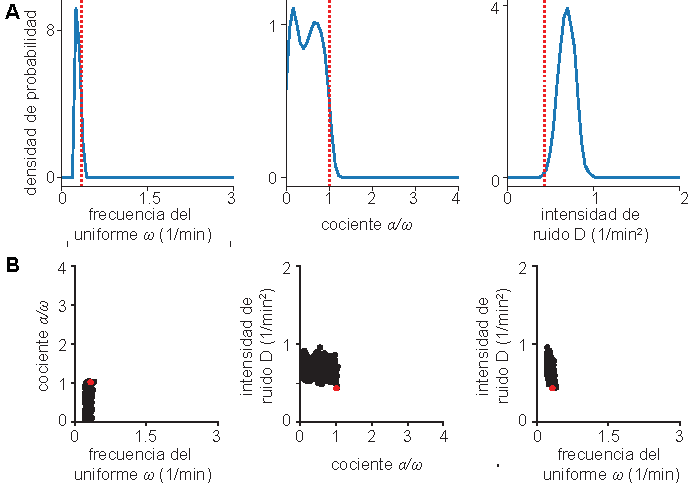
\includegraphics[width=1\columnwidth]{figures/chapter6/C6_fit_refval.pdf} 
    \caption{\textbf{Distribución \textit{posterior} obtenida como resultado del ajuste realizado con el método Cálculo Bayesiano Aproximado Monte Carlo Secuencial.} (A) Distribuciones marginales obtenidas de la \textit{posterior} que resultó del ajuste. La normalización es tal que la integral sobre todos los valores de los parámetros es 1. La linea roja punteada indica el parámetro elegido para evaluar el ajuste. (B) Proyecciones bidimensionales de los grupos de parámetros aceptados por el algoritmo ABC-SMC a partir de los cuales se estima la distribución \textit{posterior}. Los puntos rojos indican el parámetro elegido para evaluar el ajuste. (A,B) Graficamos valores de $\dddelta \geq 0$ porque decidimos restringir nuestro análisis sólo en valores positivos de los parámetros del modelo teórico. Parámetro elegido para evaluar el ajuste: $\omega = 0.33 \;\text{min}^{-1}$, $\alpha = 1.02 \times \omega$, $ D = 0.43 \; \text{min}^{-2}$ (ver apéndice \ref{C6_ap:ABC-SMC}).}
    \label{C6_fig:fit}
\end{figure} 



Como resultado, en la figura \ref{C6_fig:fit}A mostramos las distribuciones marginales de la \textit{posterior} que resultan del ajuste. Las distribuciones marginales de la frecuencia del uniforme y de la intensidad del ruido resultaron ser unimodales y angostas, sugiriendo la existencia de un rango de valores que ajustan a los datos experimentales. En particular, la moda de la distribución de frecuencias del uniforme resultó ser menor que las contempladas para estudiar la compatibilidad del modelo con las observaciones experimentales de la figura \ref{C6_fig:2d_plots_sup}. Por otro lado, la distribución marginal del cociente \dddelta asociado a la amplitud de modulación era bimodal, con un máximo en valores pequeños y otro cercanos a $1$. Si bien en la distribución marginal observamos que la mayoría de los parámetros capaz de reproducir las métricas experimentales pertenecen al régimen oscilatorio, observamos en la distribución \textit{posterior} de probabilidad conjunta que muchos de los grupos de parámetros más probables tenían valores de \dddelta mayores a uno o cercanos (apéndice \ref{C6_ap:ABC-SMC}). En la figura \ref{C6_fig:fit}B observamos las proyecciones bidimensionales de los $1000$ valores de parámetros aceptados por el modelo. Cada uno de estos puntos tiene un peso $w$ asociado, a través del cual se infiere la distribución \textit{posterior}. La convergencia del ABC-SMC promueve que en cada iteración se acepten grupos de parámetros más probables, razón por la cual se observan nubes de puntos en los rangos en donde las probabilidades marginales de los parámetros toman valores altos. 

\subsection{El modelo no logra reproducir la heterogeneidad de pulsado de los experimentos}
\label{C6_sssec:evaluac_params}

A partir de la implementación del método ABC-SMC logramos estimar la distribución \textit{posterior}, que nos informa la probabilidad de que las observaciones experimentales provengan de un dado conjunto de parámetros $(\omega,\ddelta,D)$, dadas la estadística de duración de pulsos, intervalo de interpulsado y tasa de pulsado. Esta distribución de probabilidad se infiere a partir de una muestra de $1000$ grupos de valores de parámetros a través de sus pesos $w$ (ver apéndice \ref{C6_ap:ABC-SMC}). Para continuar, evaluamos si el resultado del ajuste podía reproducir los estadísticos que utilizamos en el capítulo \ref{ch2} para definir las oscilaciones intermitentes, similar a cuando evaluamos los modelos de pulsado estocástico en la sección \ref{C2_sec:pulsado_estoctastico}. Estos estadísticos son (i) la cantidad de pulsos aislados y consecutivos, (ii) la actividad, y (iii) la frecuencia de trenes de pulsos de determinada longitud. Para realizar esta evaluación, calculamos estos tres estadísticos sobre series temporales simuladas, y comparamos el resultado con las mediciones sobre los datos experimentales. Para construir este análisis, realizamos simulaciones en donde la cantidad de trazas obtenidas era la misma que en los experimentos, y su duración similar (apéndice \ref{C6_ap:ABC-SMC}). Como el algoritmo de detección de pulsos para las simulaciones identifica el inicio, el pico y el final de cada pulso -al igual que la detección de pulsos implementada para los datos del capítulo \ref{ch2}- utilizamos las mismas estrategias que las que implementamos los datos experimentales para realizar estos cálculos. 


Los valores de máximas probabilidades marginales de cada parámetro podían representar un grupo de parámetros con baja probabilidad conjunta. Entonces, para obtener estas series temporales simuladas, elegimos uno de los $1000$ grupos de valores de parámetros $(\omega,\ddelta,D)$ que surgieron del ajuste ABC-SMC (en rojo en figura \ref{C6_fig:fit}). Como criterio, optamos por elegir un grupo de parámetros cuya probabilidad conjunta estimada por el ajuste ABC-SMC sea la más alta posible, que muchas veces no coincidía con los parámetros con probabilidades individuales altas en sus distribuciones marginales. Simultáneamente, pedimos que el grupo de parámetros elegido reproduzca la cantidad total de pulsos que observamos en los experimentos. Con esta elección, era más sencillo comparar estos observables con otras mediciones realizadas sobre nuevos modelos teóricos. Entonces, elegimos el parámetro con el mayor peso $w$ que era capaz de reproducir la cantidad total de pulsos que observamos en los experimentos (figura \ref{C6_fig:param_evaluation}, apéndice \ref{C6_ap:ABC-SMC}). 


En la figura \ref{C6_fig:param_evaluation}A observamos la estadística de la cantidad de pulsos totales, aislados o consecutivos que identificamos en los experimentos numéricos. Cada punto negro representa una de las 100 realizaciones del modelo teórico que ejecutamos para construir estadística, en donde cada realización es análoga a un experimento de $69$ células. En cada realización, contamos la cantidad de pulsos totales, aislados o consecutivos en cada una de las $69$ series temporales, y la dividimos por la duración de la traza. Luego, tomamos la mediana de las $69$ mediciones realizadas, que representamos con un punto negro en la figura. Los resultados están normalizados sobre la cantidad correspondiente detectada en los experimentos. Con esta normalización, la recta $y = 1$ (linea punteada verde) indica los valores experimentales. Como la cantidad de pulsos totales, aislados o consecutivos es discreta, en todas las realizaciones las trazas simuladas tenían la misma duración, y la normalización era la misma para todas las realizaciones en cada caso, las diferencias entre los valores representados por los puntos negros eran fijas para cada estadístico, lo que conduce a ver puntos negros organizados en lineas rectas horizontales en la figura \ref{C6_fig:param_evaluation}A. El \textit{boxplot} resume la estadística de las 100 realizaciones. Observamos que si bien el modelo reproduce la cantidad de pulsos totales, sobrestima los aislados, y subestima los consecutivos. En la figura \ref{C6_fig:param_evaluation}B observamos que el modelo es capaz de reproducir la cantidad de trenes cortos de pulsos, pero subestima fuertemente la cantidad de trenes de más de $3$ pulsos de longitud. Además, observamos que, en promedio, tanto los datos simulados como los experimentales pulsaban la misma proporción de tiempo (derecha en figura \ref{C6_fig:param_evaluation}C). Evaluando el comportamiento poblacional, si bien el modelo ajusta correctamente los valores intermedios de actividad, fallan en reproducir los casos en los que las células únicas pulsaban casi todo el tiempo de medición o no pulsaban (izquierda en figura \ref{C6_fig:param_evaluation}B). La actividad poblacional es una medida sencilla que cuantifica la heterogeneidad dinámica característica de nuestras observaciones, característica que no fue posible reproducir con el modelo teórico propuesto. Estas observaciones nos sugieren que, en el modelo teórico, los pulsos son aislados o se organizan en trenes cortos. Que el modelo logre reproducir la cantidad de pulsos totales y la actividad media es a costa de sobrestimar la cantidad de pulsos aislados, y permitir que más series temporales tengan actividad pulsátil. Como en este modelo la actividad pulsátil tiende a ser más homogénea a lo lago de la población, esto no permite reproducir la heterogeneidad de tiempo de pulsado que observamos en los experimentos. 

\begin{figure}
    \centering
    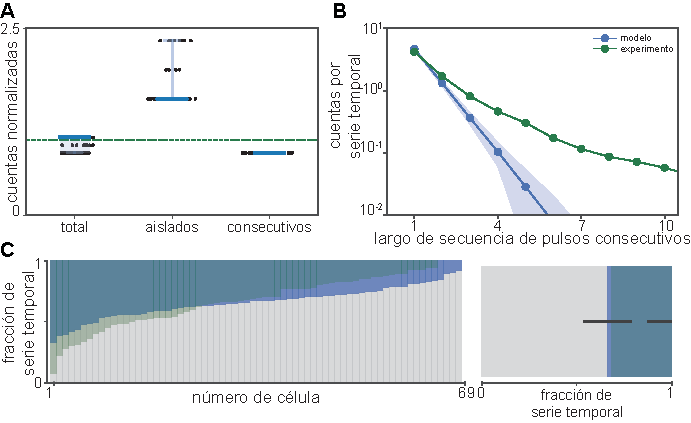
\includegraphics[width=1\columnwidth]{figures/chapter6/C6_param_evaluation.pdf} 
    \caption{\textbf{Los resultados del ajuste indican que el modelo no logra reproducir la heterogeneidad de pulsado de los experimentos.} (A) Mediana de pulsos totales, aislados y consecutivos divididos la duración de cada traza, normalizados por la mediana de las correspondientes distribuciones experimentales (puntos negros). Los datos provienen de 100 realizaciones. Las barras de color representan la mediana, los límites de la caja son los percentiles 25 y 75 de las distribuciones, y los bigotes son los percentiles 5 y 95. La linea verde referencia los valores experimentales. (B) Número de trenes de pulsos en función del número de pulsos consecutivos en el tren para las simulaciones (azul) y los datos experimentales (verde). El recuento incluye los casos que se producen dentro de trenes más largos, y el primer punto de datos corresponde al número total de pulsos individuales. Las cuentas se normalizaron por el número de series temporales. El área sombreada es desviación estándar de 100 realizaciones independientes del modelo teórico. (C) Izquierda: fracción de tiempo que las series temporales individuales pasaron pulsando (azul) o sin pulsar (gris). Derecha: tiempo medio que las series temporales estuvieron pulsando (azul) o no pulsando (gris). La barra de error indica la desviación estándar calculada sobre la población celular. En verde se indican las mediciones realizadas sobre los experimentos realizados en serum + LIF (capítulo \ref{ch2}). Estas mediciones fueron calculadas sobre 69 series temporales simuladas de 120 minutos de duración, un conjunto de datos similar al experimental. (A-C) Parámetros:  $\omega = 0.33 \;\text{min}^{-1}$, $\alpha = 1.02 \times \omega$, $ D = 0.43 \; \text{min}^{-2}$. La tasa de adquisición fue de $dt = 0.001$, cada $d = 1$ pasos. El umbral de amplitud del algoritmo de detección de pulsos fue $A_{\text{th}} = 0.9$, y la distancia umbral fue $W_{\text{th}} = 100\text{ cuadros}$. N = $69$ series temporales. $T = 120$ minutos de duración (ver apéndice \ref{C6_ap:ABC-SMC}, figura \ref{C6_ap_fig:traces_evaluation})}
    \label{C6_fig:param_evaluation}
\end{figure} 


Mostramos los histogramas de la estadística de duración de pulsos, intervalo de interpulsado y tasa de pulsado que obtuvimos a partir de las simulaciones en la figura \ref{C6_fig:dist_param_evaluation_hist}. Si bien las medianas de las distribuciones simuladas se encuentran dentro de los intervalos intercuartílicos experimentales, su distancia no responde a los valores mínimos de tolerancia del ajuste ABC-SMC (ecuación \ref{C6_eq:distancia_MC}, apéndice \ref{C6_ap:ABC-SMC}). Esto es consecuencia de generar los histogramas a partir de simulaciones con las mismas características que los datos experimentales, lo que aporta cierta variabilidad a las medianas de estos histogramas. En el caso de la duración de pulsos, obtuvimos una distribución más ancha y asimétrica que la de los datos experimentales, con valores máximos de duración más grandes, pero con valores mínimos similares. En el caso de la distribución de intervalo de interpulsado, pudimos  reproducir su asimetría característica satisfactoriamente, pero menos definida y con valores mayores. Esto probablemente sea consecuencia de subestimar la cantidad de pulsos consecutivos, responsables de los intervalos de interpulsado cortos. En el histograma de tasa de pulsado, observamos una baja proporción de series temporales sin pulsos y con muchos pulsos. Esta característica probablemente sea un reflejo tener una actividad pulsátil más homogénea en el modelo que en los experimentos. 



\begin{figure}
    \centering
    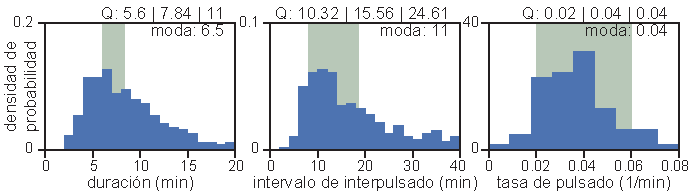
\includegraphics[width=1\columnwidth]{figures/chapter6/C6_param_evaluation_hist.pdf} 
    \caption{\textbf{Distribuciones de duración de pulsos, intervalo de interpulsado y tasa de pulsado que surgieron del ajuste del Cálculo Bayesiano Aproximado Monte Carlo Secuencial.} Distribuciones de la duración de pulsos, el intervalo de interpulsado y la tasa de pulsado, calculadas sobre 69 series temporales simuladas de 120 minutos de duración, un conjunto de datos similar al experimental. Las unidades del eje $y$ son 1/min, 1/min y min respectivamente. N = 69 células, $n_1$ = 321 pulsos, $n_2$ = 252 pares de pulsos. Los cuartiles (Q) 25, 50 y 75 y la moda se indican en la parte superior de cada gráfico. Fueron excluidos de los histogramas 5 (duración) y 22 (intervalo de interpulsado) puntos mayores que el límite del eje $x$. En verde se indica el rango intercuartílico $IQ$ correspondiente a los experimentos realizados en serum + LIF (figura \ref{C6_fig:observables_experimentales}). Parámetros: $\omega = 0.33 \;\text{min}^{-1}$, $\alpha = 1.02 \times \omega$, $ D = 0.43 \; \text{min}^{-2}$ . La tasa de adquisición fue de $dt = 0.001$, cada $d = 1$ pasos. El umbral de amplitud del algoritmo de detección de pulsos fue $A_{\text{th}} = 0.9$, y la distancia umbral fue $W_{\text{th}} = 100\text{ cuadros}$. N = $69$ series temporales. $T = 120$ minutos de duración (figura \ref{C7_fig:dist_traces_VM}).}
    \label{C6_fig:dist_param_evaluation_hist}
\end{figure} 



Como conclusión, creemos que el modelo de fase con bifurcación de ciclo infinito y ruido blanco gaussiano es insuficiente para reproducir las oscilaciones intermitentes de actividad de ERK en ESCs. Esta descripción falla en reproducir la estadística de trenes de pulsos largos, así como la heterogeneidad poblacional de la actividad pulsátil. Estos resultados sugieren que no es suficiente asumir que los pulsos son producto de excitaciones en el régimen excitable, o actividad pulsátil oscilatoria cuya coherencia se destruye con el ruido blanco gaussiano. Por otro lado, que hayamos logrado reproducir los valores intermedios de actividad que medimos en el experimento, pero con una actividad pulsátil más homogénea nos sugiere que esta heterogeneidad pueda ser descripta incorporando variabilidad de alguno de los parámetros del modelo. Motivados por estas observaciones, a continuación proponemos modificaciones al modelo teórico para mejorar la descripción teórica de nuestras observaciones experimentales. 

\section{Fluctuaciones lentas en la amplitud de modulación sobrestiman la frecuencia de trenes largos de pulsos en ausencia de ruido}
\sectionmark{Fluctuaciones lentas en la amplitud de modulación...}
%\section{La amplitud de modulación como proceso estocástico reguladora de la actividad pulsátil heterogénea}
\label{C7_sec:OU}

%motivación
En esta sección evaluamos la posibilidad de que la actividad pulsátil de ERK pueda ser descripta a partir de transiciones entre el régimen oscilatorio y el excitable descriptos por el modelo de fase con bifurcación de ciclo infinito. Con estas transiciones, esperamos obtener trenes de pulsos de mayor longitud cuando el sistema se encuentre en el régimen oscilatorio, intercalados con intervalos de silencios en el régimen excitable sin perturbar. Esperamos que transiciones cortas den lugar a pulsos aislados en la señal. Generaremos estas transiciones a partir de incorporar fluctuaciones lentas en la amplitud de modulación, y esperamos que proponer transiciones gobernadas por un proceso estocástico nos permita obtener una actividad pulsátil más heterogénea a lo largo de la población. 


\subsection{La amplitud de modulación como proceso de Ornstein-Uhlenbeck}

Proponemos modificar el modelo de fase con bifurcación de ciclo infinito de la ecuación \ref{C5_eq:adler_determinista}, y consideramos que la amplitud de modulación fluctúe lentamente a lo largo del tiempo
\begin{equation}
    \dot{\theta}(t) = \omega + \alpha_{\text{ou}}(t) \sin{(\theta(t))},
    \label{C7_eq:alpha_ou}
\end{equation}
donde $\alpha_{\text{ou}}(t)$ es un proceso de Ornstein-Uhlenbeck estacionario (OU). El ruido de Ornstein-Uhlenbeck es proceso estocástico que incorpora fluctuaciones gobernadas por una escala temporal \cite{SanMiguel2000}, donde 
\begin{align}
    \dot\alpha_{\text{ou}}(t) &= \frac{1}{\tau} (\alpha_0 - \alpha(t)) + \sqrt{\frac{2}{\tau}}\sigma \xi_w(t) \label{C7_eq:OU_langevin}\\
    \alpha_{\text{ou}}(0) &= \alpha_0.
\end{align}
Con esta definición, la estadística de la amplitud de modulación es
\begin{align}
    \langle \alpha_{\text{ou}}(t) \rangle_t &= \alpha_0 \label{C7_eq:OU_mean}\\
    \langle \alpha_{\text{ou}}(t) \; \alpha(t^\prime) \rangle_t &= \sigma^2 e^{- \lvert t-t^\prime \rvert / \tau } \label{C7_eq:OU_corr}.
\end{align}
A diferencia del ruido blanco gaussiano aditivo con el que trabajamos en el capítulo anterior, en la ecuación \ref{C7_eq:OU_langevin} podemos ver que el ruido de OU tiene un término de \textit{drift} proporcional a la diferencia entre el valor medio y el valor actual de la amplitud de modulación $\alpha_0 - \alpha_{\text{ou}}(t)$. Enfocándonos solamente en este término, observamos que si el valor actual del proceso sobrepasa su valor medio, la velocidad de la amplitud de modulación será negativa y $\alpha_{\text{ou}}(t)$ evolucionará decreciendo su valor. En cambio, si el valor actual del proceso es menor que $\alpha_0$, la velocidad será positiva y el valor del proceso crecerá. Esta característica en donde el proceso tiende siempre a desviarse hacia el valor finito $\alpha_0$ se conoce como reversión hacia la media (figura \ref{C7_fig:OU_alpha}). \marginpar{valor medio de\\ la amplitud de\\modulación} La variable $\alpha_0$ es el \textbf{valor medio de la amplitud de modulación} en el tiempo (ecuación \ref{C7_eq:OU_mean}). Al igual que la amplitud de modulación del modelo \ref{C5_eq:adler_determinista}, tiene unidades de $\text{tiempo}^{-1}$. Por simplicidad, consideraremos sólo valores positivos de $\alpha_0$. Continuando con el análisis del término de \textit{drift}, observemos que la velocidad de reversión no sólo depende de la diferencia entre el valor medio y el actual de la amplitud de modulación $\alpha_0 - \alpha(t)$, sino también la variable $\tau$.\marginpar{tiempo de\\reversión} El \textbf{tiempo de reversión} $\tau$ es la escala temporal con la que el proceso vuelve al valor medio (figura \ref{C7_fig:OU_alpha}). Por otro lado, $\xi_w(t)$ en la ecuación \ref{C7_eq:OU_langevin} representa un proceso de ruido blanco gaussiano derivado de un proceso de Wiener, que incorpora fluctuaciones instantáneas a la amplitud de modulación (ecuaciones \ref{C6_eq:wiener_mean}, \ref{C6_eq:wiener_cov}).\marginpar{volatilidad} La \textbf{volatilidad} $\sigma$ es el factor de escala de este proceso $\xi_w(t)$, que regula cuán grandes son las fluctuaciones instantáneas  (figura \ref{C7_fig:OU_alpha}). Esta variable tiene unidades de $\text{tiempo}^{-3/2}$, y consideraremos sólo valores positivos. 


\begin{figure}
    \centering
    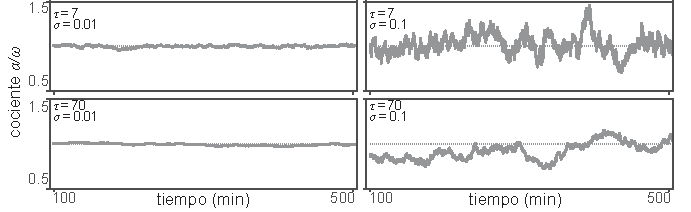
\includegraphics[width=1\columnwidth]{figures/chapter7/C7_OU_alpha.pdf} 
    \caption{\textbf{Dinámica de la amplitud de modulación como proceso de Ornstein-Uhlenbeck}. Series temporales de la amplitud de modulación en función del tiempo para distintos valores de tiempo de reversión $\tau$ y volatilidad $\sigma$ indicados en el margen superior izquierdo de cada figura, en min y $\text{min}^{-3/2}$ respectivamente. La amplitud de modulación se encuentra normalizada por una frecuencia $\omega$ constante. El valor medio de la amplitud de modulación $\alpha_0/\omega$ se encuentra representado con linea punteada. A modo de ejemplo, elegimos que el valor medio de la amplitud de modulación coincida con el punto donde aparece la bifurcación en el modelo de fase con bifurcación de ciclo infinito. Parámetros: $\alpha_0 = 2\pi/7 \;\text{ min}^{-1}$, $\omega = 2\pi/7 \;\text{ min}^{-1}$, $dt = 0.0001$, $d=10$ (apéndice \ref{C7_ap:OU_OUD_traces}).}
    \label{C7_fig:OU_alpha}
\end{figure} 

A diferencia del ruido gaussiano, cuya correlación temporal está dada por una delta de Dirac (ecuación \ref{C6_eq:wiener_cov}), la correlación temporal de la ecuación \ref{C7_eq:OU_corr} depende del tiempo de reversión $\tau$ y la volatilidad cuadrada $\sigma^2$. Esto significa que los valores del ruido en diferentes momentos no son variables aleatorias independientes, sino que están correlacionadas. A este tipo de ruidos de correlación no nula se los suele llamar ruido de color. El ruido blanco o descorrelacionado con el que trabajamos en el capítulo anterior se recupera en el límite donde $\tau \rightarrow 0$. 


%En términos sencillos, el proceso de Ornstein-Uhlenbeck es un proceso que revierte a una media $\alpha_0$ en un tiempo promedio $\tau$ y volatilidad $\sigma$. %Es un proceso gaussiano, markoviano- pues cada instante futuro del proceso está determinado únicamente por su presente y no su pasado- y estacionario- la correlación de la ecuación \ref{C7_eq:OU_corr} no depende del tiempo-.


\subsection{Fluctuaciones lentas en la amplitud de modulación producen transiciones entre oscilaciones y silencios en ausencia de ruido}
\subsectionmark{Transiciones entre oscilaciones y excitabilidad}

En el capítulo \ref{ch5} observamos que variando la amplitud de modulación del modelo de fase con bifurcación de ciclo infinito es posible transicionar entre los regímenes oscilatorio y excitable. Esta transición ocurre en el punto de bifurcación, donde la amplitud de modulación es igual a la frecuencia del uniforme. Luego, si $\alpha < \omega$, nos encontramos con el régimen oscilatorio, y si $\alpha > \omega$, en el excitable. Proponer que la amplitud de modulación varíe en el tiempo conduce a la posibilidad de transicionar entre estos dos regímenes durante la evolución del proceso. En una serie temporal de la fase $\xx(t)$, habrá momentos en donde $\alpha < \omega$ y la fase $\xx(t)$ esté oscilando, y momentos donde el sistema se encuentre en el régimen excitable cuando $\alpha > \omega$ y la fase no esté oscilando. En la circunferencia trigonométrica de radio unidad, estas posibles transiciones entre los regímenes oscilatorio y excitable que producen las fluctuaciones de la amplitud de modulación se pueden interpretar como la creación, en caso de transicionar del oscilatorio hacia el excitable, o la colisión, en caso contrario, de los puntos fijos estables e inestable. En la señal, estas transiciones reflejarán combinaciones entre actividad pulsátil y silencios, como observamos en la figura \ref{C7_fig:OU_TS}. Entonces, cuando la amplitud de modulación toma valores por debajo del punto de bifurcación, en la señal se traduce actividad pulsátil (línea gris por debajo de la línea punteada negra en la figura \ref{C7_fig:OU_TS}). En cambio, cuando tome valores por encima de este umbral, en la señal se observará un silencio (línea gris por encima de la línea punteada negra en la figura \ref{C7_fig:OU_TS}). En la figura \ref{C7_fig:OU_TS} observamos que el aumento del tiempo de reversión conduce trenes de pulsos más largos. Con la misma lógica, puede también conducir a silencios más largos. Por otro lado, el aumento de la volatilidad produce que la amplitud de modulación fluctúe instantáneamente con mayor intensidad. Fluctuaciones de mayor intensidad dan lugar a una posibilidad mayor de atravesar por un corto lapso de tiempo la bifurcación, produciendo, por ejemplo, un pulso aislado o trenes de pulsos cortos.

\begin{figure}
    \centering
    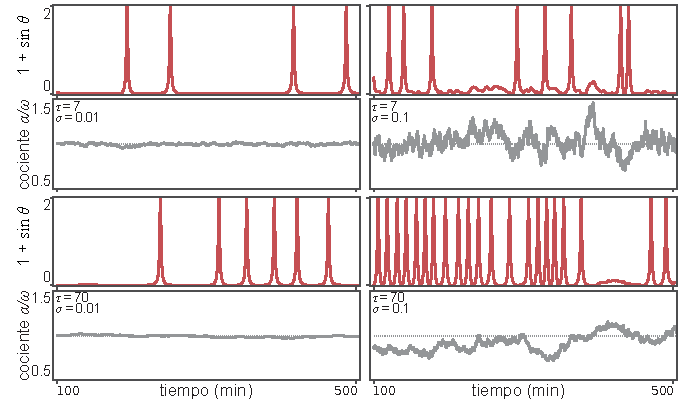
\includegraphics[width=1\columnwidth]{figures/chapter7/C7_OU_ex_traces.pdf} 
    \caption{\textbf{La amplitud de modulación como proceso de Ornstein-Uhlenbeck conduce a transiciones entre oscilaciones y silencios en ausencia de ruido.} Arriba en rojo: señal de la fase del modelo \ref{C7_eq:alpha_ou} para distintos valores de tiempo de reversión $\tau$ y volatilidad $\sigma$, indicados en min y $\text{min}^{-3/2}$ respectivamente. Abajo, en gris: la amplitud de modulación en función del tiempo correspondiente a cada señal. La amplitud de modulación se encuentra normalizada por la frecuencia frecuencia del uniforme $\omega$ constante. El valor medio de la amplitud de modulación $\alpha_0/\omega$ se encuentra representado con linea punteada. Para ejemplificar, elegimos que el valor medio de la amplitud de modulación coincida con el punto donde aparece la bifurcación en el modelo de fase con bifurcación de ciclo infinito. Parámetros:  Parámetros: $\alpha_0 = 2\pi/7 \;\text{ min}^{-1}$, $\omega = 2\pi/7 \;\text{ min}^{-1}$, $dt = 0.0001$, $d=10$ (apéndice \ref{C7_ap:OU_OUD_traces}).}
    \label{C7_fig:OU_TS}
\end{figure} 


La frecuencia del uniforme determina cuán rápido se realiza una excursión de la fase que da lugar a un pulso. Además, $\alpha_0$ determinará cuán lejos se encuentra, en promedio, la amplitud de modulación de la bifurcación y por ende está asociado a qué características del proceso estocástico son necesarias para atravesarla. Por ejemplo, un valor de $\alpha_0$ lejano a la bifurcación dará lugar a menos transiciones entre regímenes que un valor cercano. En concreto, una volatilidad pequeña es suficiente para transicionar entre regímenes en casos donde $\alpha_0$ es cercano a $\omega$, pero no cuando es muy lejano. También, para un mismo tiempo de reversión, es probable que un sistema dinámico cuyo $\alpha_0$ es es cercano a $\omega$ pase más tiempo del otro lado de la bifurcación que para un sistema dinámico cuyo $\alpha_0$ sea grande.


En definitiva, describir a la amplitud de modulación como un proceso de OU posibilita tener transiciones entre intervalos oscilatorios, silencios y pulsos aislados. Estas transiciones son características de las oscilaciones intermitentes de actividad de ERK, lo que convierte a este nuevo sistema dinámico en un buen candidato para describirlas.


\subsection{El modelo sobrestima la frecuencia de trenes de pulsos largos de los experimentos}

%2) Ajuste
Implementamos el ABC-SMC para obtener una distribución de probabilidad \textit{posterior} de los posibles $(\omega,\alpha_0,\sigma,\tau)$ que ajusten a los datos experimentales. Utilizamos la misma implementación y los mismos criterios que lo descripto en la sección \ref{C6_sssec:implementac_ABCSMC} . Las especificaciones y resultados de esta implementación se encuentran en el apéndice \ref{C6_ap:ABC-SMC}.

En la figura \ref{C7_fig:OU_fit}A podemos observar que las distribuciones marginales obtenidas son unimodales. La distribución marginal de $\alpha_0/\omega$ tiene una moda cercana a uno. Esto indica que se requieren transiciones entre los dos regímenes dinámicos con cierto dinamismo y facilidad. Es notorio que la distribución marginal de tiempo de reversión tiene un valor modal pequeño, y un segundo máximo que contempla escalas temporales más largas. En las proyecciones  bidimensionales de los grupos de parámetros aceptados por el algoritmo de ajuste de la figura \ref{C7_fig:OU_fit}B, observamos que tiempos más cortos correlacionan con mayor frecuencia con $\alpha_0$ más pequeños, cercanos a la bifurcación. 


\begin{figure}
    \centering
    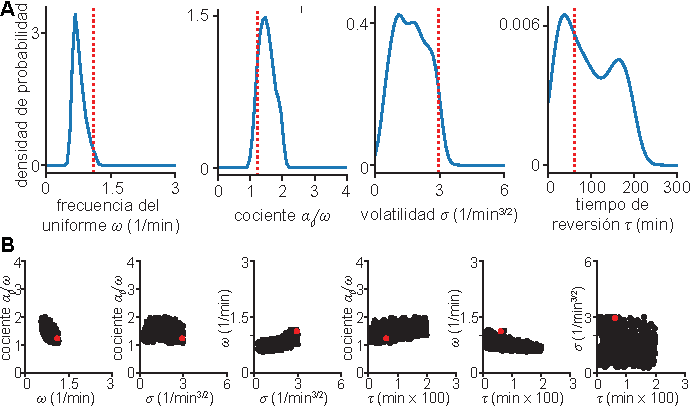
\includegraphics[width=1\columnwidth]{figures/chapter7/C7_OU_fit.pdf} 
    \caption{\textbf{Distribución \textit{posterior} obtenida como resultado del ajuste realizado con el método Cálculo Bayesiano Aproximado Monte Carlo Secuencial.} (A) Distribuciones marginales obtenidas de la \textit{posterior} que resultó del ajuste. La normalización es tal que la integral sobre todos los valores de los parámetros es 1. La linea roja punteada indica el parámetro elegido para evaluar el ajuste. (B) Proyecciones bidimensionales de los grupos de parámetros aceptados por el algoritmo ABC-SMC a partir de los cuales se estima la distribución \textit{posterior}. Los puntos rojos indican el parámetro elegido para evaluar el ajuste. (A,B) Graficamos valores de $\sigma \geq 0$ y $\tau > 0$ porque restringimos nuestro análisis a sólo valores positivos de los parámetros del modelo teórico. Parámetro elegido para evaluar el ajuste: $\omega = 1.11\; \text{min}^{-1}$, $\alpha_0 = 1.23 \times \omega$, $ \sigma = 2.94 \;  \text{min}^{-3/2}$ y $\tau = 61.02 \; \text{min} $ (ver apéndice \ref{C7_ap:ABC-SMC}, figura \ref{C7_fig:ap_eps}).}
    \label{C7_fig:OU_fit}
\end{figure} 


%pulsos aislados y consecutivos
%validación
Evaluamos si el resultado del ajuste podía reproducir los estadísticos que describen las oscilaciones intermitentes, realizando la misma comparación que en la sección \ref{C6_sssec:evaluac_params}. Los valores de $(\omega,\alpha_0,\sigma,\tau)$ con los que elegimos trabajar se encuentran indicados en rojo en la figura \ref{C7_fig:OU_fit}, y fueron elegidos con los criterios que definimos previamente. Observamos que el modelo es capaz de reproducir correctamente la cantidad de pulsos totales, pero en este caso sobrestima los consecutivos y subestima los aislados (figura \ref{C7_fig:OU_param_evaluation}A). Esta diferencia se traduce en una mayor cantidad de trenes de pulsos que las adquiridas en las observaciones experimentales (figura \ref{C7_fig:OU_param_evaluation}B). A diferencia del modelo anterior, en la figura \ref{C7_fig:OU_param_evaluation}C observamos que este nuevo modelo puede ajustar correctamente los casos en los que las células únicas pulsaban casi todo el tiempo de medición o no pulsaban, reproduciendo satisfactoriamente la heterogeneidad de nuestras observaciones, al igual que la proporción de tiempo promedio en que las células pulsaban.

\begin{figure}
    \centering
    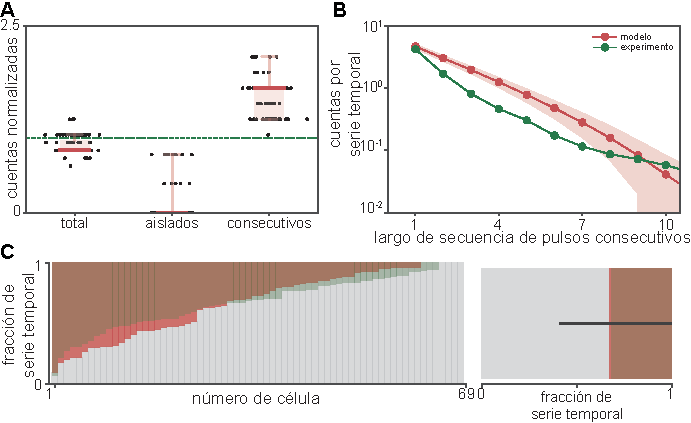
\includegraphics[width=1\columnwidth]{figures/chapter7/C7_OU_validation.pdf} 
    \caption{\textbf{Los resultados del ajuste indican que el modelo sobrestima la frecuencia de trenes largos de pulsos.} (A) Mediana de pulsos totales, aislados y consecutivos divididos la duración de cada traza, normalizados por la mediana de las correspondientes distribuciones experimentales (puntos negros). Los datos provienen de 100 realizaciones. Las barras de color representan la mediana, los límites de la caja son los percentiles 25 y 75 de las distribuciones, y los bigotes son los percentiles 5 y 95. La linea verde referencia los valores experimentales. (B) Número de trenes de pulsos en función del número de pulsos consecutivos en el tren para las simulaciones (rojo) y los datos experimentales (verde). El recuento incluye los casos que se producen dentro de trenes más largos, y el primer punto de datos corresponde al número total de pulsos individuales. Las cuentas se normalizaron por el número de series temporales. El área sombreada es desviación estándar de 100 realizaciones independientes del modelo teórico. (C) Izquierda: fracción de tiempo que las series temporales individuales pasaron pulsando (rojo) o sin pulsar (gris). Derecha: Tiempo medio que las series temporales estuvieron pulsando (rojo) o no pulsando (gris). La barra de error indica la desviación estándar calculada sobre la población celular. En verde se indican las mediciones realizadas sobre los experimentos realizados en serum + LIF (capítulo \ref{ch2}). Estas mediciones fueron calculadas sobre 69 series temporales simuladas de 120 minutos de duración, un conjunto de datos similar al experimental. (A-C) Parámetros: $\omega = 1.11 \; \text{min}^{-1}$, $\alpha_0 = 1.23 \times \omega$, $ \sigma = 2.94 \; \; \text{min}^{-3/2}$ y $\tau = 61.02 \; \text{min} $ (ver apéndice \ref{C6_ap:ABC-SMC}). La tasa de adquisición fue de $dt = 0.001$, cada $d = 1$ pasos. El umbral de amplitud del algoritmo de detección de pulsos fue $A_{\text{th}} = 0.9$, y la distancia umbral fue $W_{\text{th}} = 100\text{ cuadros}$. N = $69$ series temporales. $T = 120$ minutos de duración (figura \ref{C7_fig:OU_traces_VM}).}
    \label{C7_fig:OU_param_evaluation}
\end{figure} 

Los histogramas de la estadística de duración de pulsos, intervalo de interpulsado y tasa de pulsado se encuentran en la figura \ref{C7_fig:OU_param_evaluation_hist}. En el caso de la duración de pulsos, obtuvimos en promedio duraciones más cortas que los experimentos, pero con algunas duraciones más largas. Para los intervalos de interpulsado, fue posible reproducir su asimetría característica satisfactoriamente, pero trasladada hacia valores menores. El haber logrado reproducir esta asimetría probablemente esté relacionado a reproducir la actividad heterogénea experimental. Que la distancia entre el primer cuartil y la media sea notoriamente más pequeña que en los experimentos está posiblemente asociado a más frecuencia de trenes de pulsos de mayor longitud en las series temporales simuladas. Además, que los intervalos de interpulsado sean en general más cortos puede estar correlacionado con tener menores duraciones de los pulsos. Finalmente, en la tasa de pulsado vemos que hay más células que no pulsan que en los experimentos, efecto que también se puede observar en el panel de la izquierda la figura \ref{C7_fig:OU_param_evaluation}C. Sin embargo, se observa una distribución menos definida que la del capítulo anterior, más parecida a la experimental y reflejando, una vez más, la heterogeneidad de actividad pulsátil. 

\begin{figure}
    \centering
    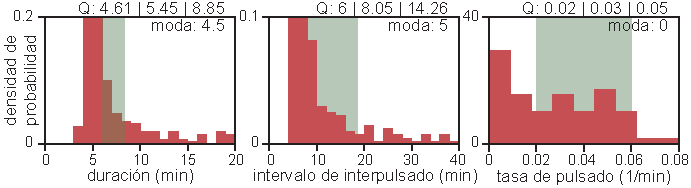
\includegraphics[width=1\columnwidth]{figures/chapter7/C7_OU_validation_hist.pdf} 
    \caption{\textbf{Distribuciones de duración de pulsos, intervalo de interpulsado y tasa de pulsado que surgieron del ajuste del Cálculo Bayesiano Aproximado Monte Carlo Secuencial.} (A) Distribuciones de la duración de pulsos, el intervalo de interpulsado y la tasa de pulsado, calculadas sobre 69 series temporales simuladas de 120 minutos de duración, un conjunto de datos similar al experimental. Las unidades del eje $y$ son 1/min, 1/min y min respectivamente. N = 69 células, $n_1$ = 275 pulsos, $n_2$ = 213 pares de pulsos. Los cuartiles (Q) 25, 50 y 75 y la moda se indican en la parte superior de cada gráfico. Fueron excluidos de los histogramas 27 (duración), 12 (intervalo de interpulsado) y 4 (tasa de pulsado) puntos mayores que el límite del eje $x$. En verde se indica el rango intercuartílico $IQ$ correspondiente a los experimentos realizados en serum + LIF (figura \ref{C6_fig:observables_experimentales}). Parámetros: $\omega = 1.11\; \text{min}^{-1}$, $\alpha_0 = 1.23 \times \omega$, $ \sigma = 2.94 \; \text{min}^{-3/2}$ y $\tau = 61.02 \; \text{min} $ (ver apéndice \ref{C7_ap:ABC-SMC}). La tasa de adquisición fue de $dt = 0.001$, cada $d = 1$ pasos. El umbral de amplitud del algoritmo de detección de pulsos fue $A_{\text{th}} = 0.9$, y la distancia umbral fue $W_{\text{th}} = 100\text{ cuadros}$. N = $69$ series temporales. $T = 120$ minutos de duración (figura \ref{C7_fig:OU_traces_VM}).}
    \label{C7_fig:OU_param_evaluation_hist}
\end{figure} 


En definitiva, incorporar fluctuaciones lentas en la amplitud de modulación describiéndola como un proceso de OU conduce a reproducir satisfactoriamente la actividad pulsátil heterogénea que observamos en las series temporales de actividad de ERK. Sin embargo, contrariamente al primer modelo considerado, este modelo teórico sobrestima la cantidad de pulsos consecutivos del experimento y subestima los aislados, conduciendo a una frecuencia más alta de trenes de pulsos largos. Esto demuestra que generar transiciones entre el régimen oscilatorio -produciendo oscilaciones- y el excitable -produciendo intervalos de silencio- de la manera propuesta es suficiente para reproducir trenes de pulsos largos, pero no para describir los pulsos aislados, reforzando la idea de que estos pulsos aislados son signos de excitabilidad. 


\section{Fluctuaciones lentas en la amplitud de modulación describen las oscilaciones intermitentes en presencia de ruido}
\sectionmark{Fluctuaciones lentas en la amplitud de modulación con ruido...}
\label{C7_sec:OUD}
%0) motivacion para proponer ESTE nuevo modelo (excitabilidad)

Los resultados previos sugieren la idea de que los trenes de pulsos que observamos reflejen actividad oscilatoria de ERK, y los pulsos aislados sean reminiscencias de excitabilidad. En esta sección proponemos una modificación al modelo teórico para poner a prueba esta interpretación. Proponemos un sistema dinámico que presente transiciones entre un régimen dinámico oscilatorio y uno excitable, y a la vez haya perturbaciones que potencialmente darán lugar a actividad pulsátil en el excitable. Esperamos que estas modificaciones permitan reproducir la proporción de pulsos aislados de los experimentos. 


\subsection{Fluctuaciones lentas en la amplitud de modulación y ruido blanco gaussiano aditivo producen transiciones entre oscilaciones y excitabilidad}

Proponemos incluir en el modelo de fase con bifurcación de ciclo infinito dos modificaciones: (i) describir a la amplitud de modulación como un proceso de Ornstein-Uhlenbeck, e (ii) incorporar ruido blanco gaussiano aditivo
\begin{equation}
    \dot{\theta}(t) = \omega + \alpha_{\text{ou}}(t) \sin{(\theta(t))} + \sqrt{2D} \xi_w(t).
    \label{C7_eq:alpha_ou_D}
\end{equation}
Con esta descripción, esperamos que el ruido de OU en $\alpha_{\text{ou}}(t)$ nos conduzca a tener transiciones entre los dos regímenes dinámicos (ecuaciones \ref{C7_eq:OU_langevin}, \ref{C7_eq:VM}, \ref{C7_eq:OU_corr}). A partir de nuestras observaciones previas del capítulo anterior, esperamos que durante estas transiciones el ruido blanco gaussiano aditivo $\sqrt{2D} \xi_w(t)$ tienda a desordenar las oscilaciones en el régimen oscilatorio, y a la promover la actividad pulsátil en el régimen excitable (ecuaciones \ref{C6_eq:wiener_mean}, \ref{C6_eq:wiener_cov}). 


\subsection{El modelo reproduce las principales características dinámicas que describen las oscilaciones intermitentes de los experimentos}

%2) Ajuste
Implementamos el ABC-SMC para obtener una distribución de probabilidad \textit{posterior} de los posibles $(\omega,\alpha_0,\sigma,\tau,D)$ que ajusten a los datos experimentales. Utilizamos la misma implementación y criterios que en la sección \ref{C6_sssec:implementac_ABCSMC}. Las especificaciones y resultados de esta implementación se encuentran en el apéndice \ref{C7_ap:ABC-SMC}.


\begin{figure}
    \centering
    \includegraphics[width=1\columnwidth]{figures/chapter7/C7_OUD_fit.pdf} 
    \caption{\textbf{Distribución \textit{posterior} obtenida como resultado del ajuste realizado con el método Cálculo Bayesiano Aproximado Monte Carlo Secuencial.} (A) Distribuciones marginales obtenidas de la \textit{posterior} que resultó del ajuste. La normalización es tal que la integral sobre todos los valores de los parámetros es 1. La linea roja punteada indica el parámetro elegido para evaluar el ajuste. (B) Proyecciones bidimensionales de los grupos de parámetros aceptados por el algoritmo ABC-SMC a partir de los cuales se estima la distribución \textit{posterior}. Los puntos rojos indican el parámetro elegido para evaluar el ajuste. (A,B) Graficamos valores de $\alpha_0 / \omega \geq 0$ , $\sigma  \geq 0$, $\tau  > 0$ y $D  \geq 0$ porque restringimos nuestro análisis sólo en valores positivos de los parámetros del modelo teórico. Parámetro elegido para evaluar el ajuste: $\omega = 0.65 \; \text{min}^{-1}$, $\alpha_0 = 1.08 \times \omega$, $ \sigma = 0.45 \; \; \text{min}^{-3/2}$, $\tau = 142.06 \; \text{min} $ y $D = 0.11 \; \; \text{min}^{-2}$ (ver apéndice \ref{C7_ap:ABC-SMC}, figura \ref{C7_fig:ap_eps}).}
    \label{C7_fig:OUD_fit}
\end{figure} 


En la figura \ref{C7_fig:OUD_fit} podemos observar que las distribuciones marginales obtenidas son unimodales. La distribución marginal de $\alpha_0/\omega$ tiene una moda es cercana a al valor unidad, al igual que en el caso anterior. La volatilidad toma valores más grandes, y el tiempo de reversión consiste en escalas temporales más largas comparadas con el ajuste previo. En este caso la distribución del tiempo de correlación tiene un sólo máximo. Esto sugiere que en el caso anterior las dos escalas temporales modales que observamos posiblemente provengan de intentar describir simultáneamente dos regímenes distintos de pulsado. Por otro lado, la distribución marginal de la intensidad del ruido está bien definida, y toma valores más pequeños en comparación al modelo de la sección \ref{C6_sec:alder_ruido_fit}. Es posible que esta diferencia consista en que en este modelo el rol del ruido sea principalmente perturbar el régimen excitable, y no competir con el modelo determinista para dominar la dinámica. 

%pulsos aislados y consecutivos
Evaluamos si el resultado del ajuste podía reproducir los estadísticos que describen las oscilaciones intermitentes realizando la misma comparación que en la sección \ref{C6_sssec:evaluac_params}. Los valores de $(\omega,\alpha_0,\sigma,\tau,D)$ con los que elegimos trabajar en esta sección se encuentran indicados en rojo en la figura \ref{C7_fig:OUD_fit}, y fueron elegidos con los criterios que definimos previamente. Observamos que el modelo reproduce correctamente la cantidad de pulsos totales y aislados, y en promedio subestima levemente los consecutivos (figura \ref{C7_fig:OUD_param_evaluation}A). Este resultado se condice con la cantidad de trenes de pulsos de determinada duración, donde observamos que las simulaciones reproducen satisfactoriamente la tendencia del comportamiento, incluso hasta la frecuencia de trenes largos de hasta $8$ pulsos (figura \ref{C7_fig:OUD_param_evaluation}B). Además, este modelo ajusta los casos en los que las células únicas pulsaban casi todo el tiempo de medición o no pulsaban, y reproduce satisfactoriamente tanto la heterogeneidad de nuestras observaciones, como la proporción de tiempo en que las células pulsaban en promedio (figura \ref{C7_fig:OUD_param_evaluation}C). La leve diferencia  entre el modelo y los experimentos en los valores altos de actividad de células únicas posiblemente esté asociado a la presencia de trenes de $9$ o más pulsos, así como la leve subestimación de la cantidad de pulsos consecutivos. 


\begin{figure}
    \centering
    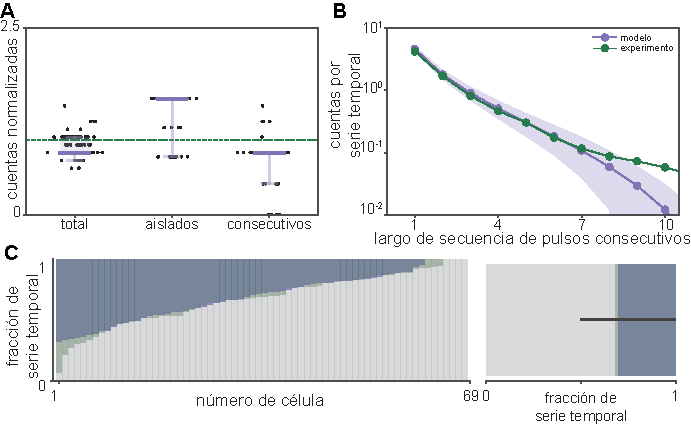
\includegraphics[width=1\columnwidth]{figures/chapter7/C7_OUD_validation.pdf} 
    \caption{\textbf{Los resultados del ajuste indican que el modelo logra describir las oscilaciones intermitentes.} (A) Mediana de pulsos totales, aislados y consecutivos divididos la duración de cada traza, normalizados por la mediana de las correspondientes distribuciones experimentales (puntos negros). Los datos provienen de 100 realizaciones. Las barras de color representan la mediana, los límites de la caja son los percentiles 25 y 75 de las distribuciones, y los bigotes son los percentiles 5 y 95. La linea verde referencia los valores experimentales. (B) Número de trenes de pulsos en función del número de pulsos consecutivos en el tren para las simulaciones (violeta) y los datos experimentales (verde). El recuento incluye los casos que se producen dentro de trenes más largos, y el primer punto de datos corresponde al número total de pulsos individuales. Las cuentas se normalizaron por el número de series temporales. El área sombreada es desviación estándar de 100 realizaciones independientes del modelo teórico. (C) Izquierda: fracción de tiempo que las series temporales individuales pasaron pulsando (violeta) o sin pulsar (gris). Derecha: tiempo medio que las series temporales estuvieron pulsando (violeta) o no pulsando (gris). La barra de error indica la desviación estándar medida sobre la población celular. En verde se indican las mediciones realizadas sobre los experimentos realizados en serum + LIF (capítulo \ref{ch2}). Estas mediciones fueron calculadas sobre 69 series temporales simuladas de 120 minutos de duración, un conjunto de datos similar al experimental. (A-C) Parámetros:  $\omega = 0.65 \; \text{min}^{-1}$, $\alpha_0 = 1.08 \times \omega$, $ \sigma = 0.45 \; \text{min}^{-3/2}$, $\tau = 142.06 \; \text{min} $ y $D = 0.11 \; \text{min}^{-2}$ (ver apéndice \ref{C7_ap:ABC-SMC}). La tasa de adquisición fue de $dt = 0.001$, cada $d = 1$ pasos. El umbral de amplitud del algoritmo de detección de pulsos fue $A_{\text{th}} = 0.9$, y la distancia umbral fue $W_{\text{th}} = 100\text{ cuadros}$. N = $69$ series temporales. $T = 120$ minutos de duración (figura \ref{C7_fig:OUD_traces_VM}).}
    \label{C7_fig:OUD_param_evaluation}
\end{figure} 


Los histogramas de la estadística de duración de pulsos, intervalo de interpulsado y tasa de pulsado se encuentran en la figura \ref{C7_fig:OUD_param_evaluation_hist}. Observamos que la estadística de duración de pulsos se ajusta razonablemente, tantos sus estadísticos como su forma. En el caso de la distribución de intervalo de interpulsado, pudimos también reproducir sus estadísticos. Además, logramos ajustar la forma de la distribución, aunque su cola fue levemente más corta en el ajuste. Posiblemente esta discrepancia esté correlacionada con la leve diferencia que observamos en la figura \ref{C7_fig:OUD_param_evaluation}C, donde se ve que en las simulaciones hay más células sin actividad pulsátil que en los experimentos. En la distribución de tasa de pulsado podemos ver que esta diferencia es más pequeña que en el caso de la sección anterior, donde el modelo no tenía ruido blanco aditivo. 


\begin{figure}
    \centering
    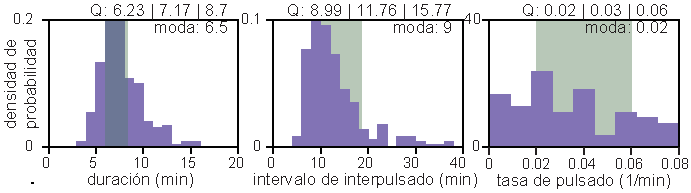
\includegraphics[width=1\columnwidth]{figures/chapter7/C7_OUD_validation_hist.pdf} 
    \caption{\textbf{Distribuciones de duración de pulsos, intervalo de interpulsado y tasa de pulsado que surgieron del ajuste del Cálculo Bayesiano Aproximado Monte Carlo Secuencial.} (A) Distribuciones de la duración de pulsos, el intervalo de interpulsado y la tasa de pulsado, calculadas sobre 69 series temporales simuladas de 120 minutos de duración, un conjunto de datos similar al experimental.Las unidades del eje $y$ son 1/min, 1/min y min respectivamente. N = 69 células, $n_1$ = 333 pulsos, $n_2$ = 271 pares de pulsos. Los cuartiles (Q) 25, 50 y 75 y la moda se indican en la parte superior de cada gráfico. Fueron excluidos de los histogramas 15 (intervalo de interpulsado) y 7 (tasa de pulsado) puntos mayores que el límite del eje $x$. En verde se indica el rango intercuartílico $IQ$ correspondiente a los experimentos realizados en serum + LIF (figura \ref{C6_fig:observables_experimentales}). Parámetros:  $\omega = 0.65 \; \text{min}^{-1}$, $\alpha_0 = 1.08 \times \omega$, $ \sigma = 0.45 \; \; \text{min}^{-3/2}$, $\tau = 142.06 \; \text{min} $ y $D = 0.11 \; \; \text{min}^{-2}$ (ver apéndice \ref{C7_ap:ABC-SMC}). La tasa de adquisición fue de $dt = 0.001$, cada $d = 1$ pasos. El umbral de amplitud del algoritmo de detección de pulsos fue $A_{\text{th}} = 0.9$, y la distancia umbral fue $W_{\text{th}} = 100\text{ cuadros}$. N = $69$ series temporales. $T = 120$ minutos de duración (figura \ref{C7_fig:OUD_traces_VM}).}
    \label{C7_fig:OUD_param_evaluation_hist}
\end{figure} 


En resumen, tener simultáneamente transiciones entre el régimen oscilatorio y el excitable, y ruido blanco gaussiano aditivo capaz de generar actividad pulsátil en el régimen excitable es capaz de producir intervalos oscilatorios intercalados con intervalos de silencios y pulsos aislados. Con estos resultados, creemos que este modelo teórico es suficiente para describir las principales características dinámicas de las oscilaciones intermitentes de ERK en ESCs. Además, encontramos que es posible generar oscilaciones intermitentes con escalas temporales similares a las que medimos en los experimentos. Observamos en la figura \ref{C7_fig:OUD_fit}A que existen tiempos de reversión largos en los resultados del ajuste, que son comparables con la duración de nuestras mediciones experimentales de aproximadamente 2 horas. Con estos tiempos, es posible que el sistema dinámico se encuentre en un sólo régimen dinámico durante toda la medición y se pueda considerar a la amplitud de modulación como estacionaria. En estos hipotéticos casos en donde la amplitud de modulación es estacionaria, podríamos prescindir de incorporar una escala temporal para describir sus fluctuaciones. En la próxima sección evaluamos esta idea.


\section{Fluctuaciones estacionarias en la amplitud de modulación subestiman la frecuencia de trenes largos de pulsos en ausencia de ruido}
\sectionmark{Fluctuaciones estacionarias en la amplitud de modulación con ruido...}
\label{C7_sec:dist}

%motivación
Motivados por los resultados previos, en esta sección evaluamos la posibilidad de que las fluctuaciones que representamos en la amplitud de modulación puedan ser incorporadas como procesos estacionarios en cada serie temporal. Con esta hipótesis, la amplitud de modulación tomaría un valor fijo constante, y en principio distinto para cada célula. A partir de esta descripción, esperamos poder evaluar si es posible prescindir de incorporar una escala temporal para describir las fluctuaciones de la amplitud de modulación.


\subsection{La amplitud de modulación muestreada de una distribución gaussiana produce oscilaciones o excitabilidad}
\subsectionmark{La amplitud de modulación muestreada de una distribución gaussiana}

Consideraremos el modelo de fase de bifurcación de ciclo infinito y ruido blanco gaussiano aditivo
\begin{equation}
    \dot{\theta_i}(t) = \omega + \alpha_i \sin{(\theta_i(t))}+ \sqrt{2D} \xi_w(t),
\end{equation}
en donde $i$ es el índice celular. Con esta descripción, cada medición tendrá una amplitud de modulación $\alpha_i$ fija y, en principio, diferente. Además, cada medición de una célula $i$ tendrá una trayectoria propia $\theta_i(t)$. 


Describir a cada célula con un valor distinto de la amplitud de modulación implica que cada una de las trayectorias del sistema dinámico tenga la posibilidad de estar en un régimen dinámico diferente. En los casos en donde $\alpha_i < \omega$, las trayectorias de la fase serán oscilatorias, y el ruido destruirá la coherencia de las oscilaciones. Cuando $\alpha_i > \omega$, el sistema estará en el régimen excitable, y existe la posibilidad de que el ruido perturbe al sistema y genere actividad pulsátil. Proponemos adquirir a la amplitud de modulación de una distribución gaussiana de media $\mu_{\alpha}$ y desviación estándar $\sigma_{\alpha}$ en cada medición. Como restringimos el análisis a valores no negativos de la amplitud de modulación, truncamos en cero esta distribución (figura \ref{C7_fig:dist_def}).


\begin{figure}
    \centering
    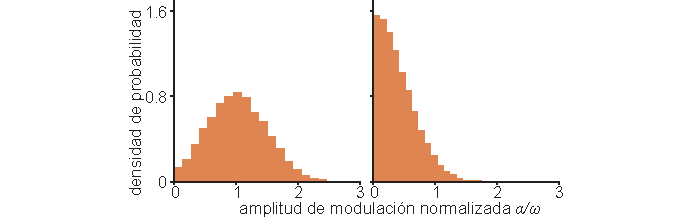
\includegraphics[width=1\columnwidth]{figures/chapter7/C7_dist_def.pdf} 
    \caption{\textbf{Los valores de la amplitud de modulación son muestreados de una distribución.} Posibles distribuciones de muestreo gaussianas truncadas de la amplitud de modulación. Izquierda: $\mu_{\alpha} = 1 \; \text{min}^{-1}$. Derecha: $\mu_{\alpha} = 0$. En ambos casos $\sigma_{\alpha} = 0.5 \; \text{min}^{-1}$ y N = 10000. }
    \label{C7_fig:dist_def}
\end{figure} 


\subsection{El modelo subestima la frecuencia de trenes de pulsos largos}

%2) Ajuste
Implementamos el ABC-SMC para obtener una distribución de probabilidad \textit{posterior} de los posibles $(\omega,\mu_{\alpha},\sigma_{\alpha},D)$ que ajusten a los datos experimentales. Utilizamos la misma implementación y criterios que en la sección \ref{C6_sssec:implementac_ABCSMC}. Las especificaciones y resultados de esta implementación se encuentran en el apéndice \ref{C7_ap:ABC-SMC}.


\begin{figure}
    \centering
    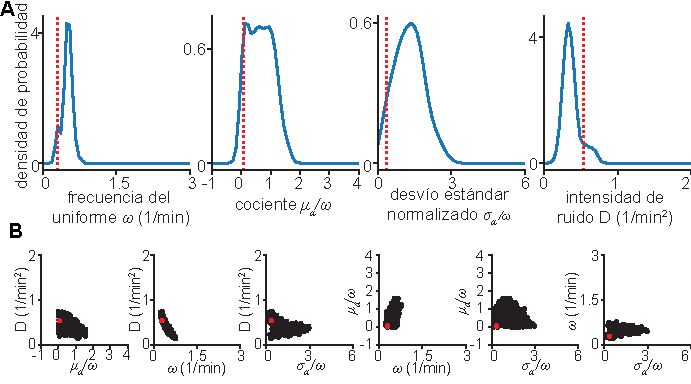
\includegraphics[width=1\columnwidth]{figures/chapter7/C7_dist_fit.pdf} 
    \caption{\textbf{Distribución \textit{posterior} obtenida como resultado del ajuste realizado con el método Cálculo Bayesiano Aproximado Monte Carlo Secuencial.} (A) Distribuciones marginales obtenidas de la \textit{posterior} que resultó del ajuste. La normalización es tal que la integral sobre todos los valores de los parámetros es 1. La linea roja punteada indica el parámetro elegido para evaluar el ajuste. (B) Proyecciones bidimensionales de los grupos de parámetros aceptados por el algoritmo ABC-SMC a partir de los cuales se estima la distribución \textit{posterior}. Los puntos rojos indican el parámetro elegido para evaluar el ajuste. (A,B) Graficamos valores de $\sigma_{\alpha}  > 0$ porque definimos el desvío estándar positivo. Parámetro elegido para evaluar el ajuste: $\omega = 0.23 \; \text{min}^{-1}$, $\mu_{\alpha} = 0.06 \times \omega$, $ \sigma_{\alpha} = 0.36 \;  \times \omega $ y $D = 0.54 \;\text{min}^{-2}$ (ver apéndice \ref{C7_ap:ABC-SMC}, figura \ref{C7_fig:ap_eps}).}
    \label{C7_fig:dist_fit}
\end{figure} 


En la figura \ref{C7_fig:dist_fit}A podemos observar que las distribuciones marginales obtenidas son unimodales. En particular, la distribución marginal del valor medio de la distribución de muestreo de la amplitud de modulación normalizado por la frecuencia del uniforme está centrada en uno, y la del desvío estándar normalizado presenta valores comparables. En la figura \ref{C7_fig:dist_fit}B observamos que para valores medios pequeños, el ancho de la distribución puede ser más grande, y para valores medios más grandes, la distribución de la amplitud de modulación es más definida. Esto sugiere que para reproducir la estadística de los observables de la dinámica de actividad de ERK, posiblemente sean necesarios valores altos de la amplitud de modulación que conduzcan al régimen excitable, y valores pequeños que lo hagan al oscilatorio.  

%pulsos aislados y consecutivos
Evaluamos si el resultado del ajuste podía reproducir los estadísticos que describen las oscilaciones intermitentes, realizando la misma comparación que en la sección \ref{C6_sssec:evaluac_params}. Los valores de $(\omega,\mu_{\alpha},\sigma_{\alpha},D)$ con los que elegimos trabajar en esta sección se encuentran indicados en rojo en la figura \ref{C7_fig:dist_fit}, y fueron elegidos con los criterios que definimos previamente. Observamos en la figura \ref{C7_fig:dist_param_evaluation}A que cuando modelo reproduce correctamente la cantidad de pulsos totales, subestima la cantidad de pulsos consecutivos y sobrestima los aislados. Al igual que en en la sección \ref{C6_sec:alder_ruido_fit}, esto conduce a subestimar la frecuencia de trenes de pulsos largos (figura \ref{C7_fig:dist_param_evaluation}B). Sin embargo, es interesante que el modelo reproduce satisfactoriamente la heterogeneidad de nuestras observaciones de actividad (figura \ref{C7_fig:dist_param_evaluation}C). Observamos gran similitud entre la actividad poblacional en el modelo y los experimentos, incluso en los casos en los que las células no pulsan o pulsan a lo largo de casi toda la medición. Como anteriormente, este ajuste se ve acompañado por el ajuste de la actividad media poblacional.


\begin{figure}
    \centering
    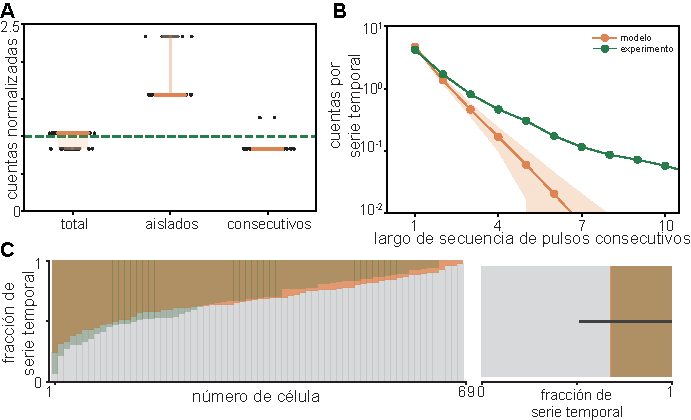
\includegraphics[width=1\columnwidth]{figures/chapter7/C7_dist_validation.pdf} 
    \caption{\textbf{Los resultados del ajuste indican que el modelo subestima la frecuencia de trenes de pulsos largos.} (A) Mediana de pulsos totales, aislados y consecutivos divididos la duración de cada traza, normalizados por la mediana de las correspondientes distribuciones experimentales (puntos negros). Los datos provienen de 100 realizaciones. Las barras de color representan la mediana, los límites de la caja son los percentiles 25 y 75 de las distribuciones, y los bigotes son los percentiles 5 y 95. La linea verde referencia los valores experimentales. (B) Número de trenes de pulsos en función del número de pulsos consecutivos en el tren para las simulaciones (naranja) y los datos experimentales (verde). El recuento incluye los casos que se producen dentro de trenes más largos, y el primer punto de datos corresponde al número total de pulsos individuales. Las cuentas se normalizaron por el número de series temporales. El área sombreada es desviación estándar de 100 realizaciones independientes del modelo teórico. (C) Izquierda: fracción de tiempo que las series temporales individuales pasaron pulsando (naranja) o sin pulsar (gris). A la derecha: Tiempo medio que las series temporales estuvieron pulsando (naranja) o no pulsando (gris). La barra de error indica la desviación estándar calculada sobre la población celular. En verde se indican las mediciones realizadas sobre los experimentos realizados en serum + LIF (capítulo \ref{ch2}). Estas mediciones fueron calculadas sobre 69 series temporales simuladas de 120 minutos de duración, un conjunto de datos similar al experimental. (A-C) Parámetros:  $\omega = 0.30 \; \text{min}^{-1}$, $\mu_{\alpha} = 0.06 \times \omega$, $ \sigma_{\alpha} = 0.36 \times \omega$ y $D = 0.54 \;  \; \text{min}^{-2}$ (ver apéndice \ref{C7_ap:ABC-SMC}). La tasa de adquisición fue de $dt = 0.001$, cada $d = 1$ pasos. El umbral de amplitud del algoritmo de detección de pulsos fue $A_{\text{th}} = 0.9$, y la distancia umbral fue $W_{\text{th}} = 100\text{ cuadros}$. N = $69$ series temporales. $T = 120$ minutos de duración (figura \ref{C7_fig:dist_traces_VM}).}
    \label{C7_fig:dist_param_evaluation}
\end{figure} 



Los histogramas de la estadística de duración de pulsos, intervalo de interpulsado y tasa de pulsado se encuentran en la figura \ref{C7_fig:dist_param_evaluation_hist}. Si bien la estadística de duración de pulsos se ajusta razonablemente, su forma demuestra que hay una mayor variabilidad en las duraciones de pulsos del modelo que del experimento. Previamente estudiamos que la duración de pulsos depende de la amplitud de modulación. Estos resultados sugieren que valores altos de desvío estándar de la distribución de muestreo de $\alpha_i$ conduzcan a distribuciones de duración de pulsos anchas.  La variabilidad observada en la distribución de duración de pulsos también se observa en la distribución de intervalos de interpulsado.


\begin{figure}
    \centering
    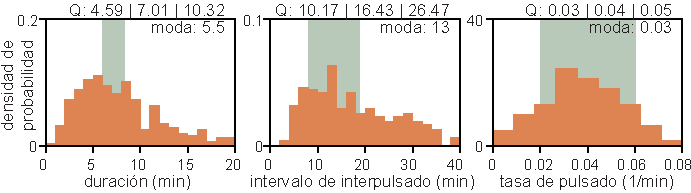
\includegraphics[width=1\columnwidth]{figures/chapter7/C7_dist_validation_hist.pdf} 
    \caption{\textbf{Distribuciones de duración de pulsos, intervalo de interpulsado y tasa de pulsado que surgieron del ajuste del Cálculo Bayesiano Aproximado Monte Carlo Secuencial.} Distribuciones de la duración de pulsos, el intervalo de interpulsado y la tasa de pulsado, calculadas sobre 69 series temporales simuladas de 120 minutos de duración, un conjunto de datos similar al experimental. Las unidades del eje $y$ son 1/min, 1/min y min respectivamente. N = 69 células, $n_1$ = 327 pulsos, $n_2$ = 258 pares de pulsos. Los cuartiles (Q) 25, 50 y 75 y la moda se indican en la parte superior de cada gráfico. Fueron excluidos de los histogramas 9 (duración) y 19 (intervalo de interpulsado) puntos mayores que el límite del eje $x$. En verde se indica el rango intercuartílico $IQ$ correspondiente a los experimentos realizados en serum + LIF (figura \ref{C6_fig:observables_experimentales}). Parámetros:  $\omega = 0.30 \; \text{min}^{-1}$, $\mu_{\alpha} = 0.06 \times \omega$, $ \sigma_{\alpha} = 0.36  \times \omega$ y $D = 0.54 \; \text{min}^{-2}$ (ver apéndice \ref{C7_ap:ABC-SMC}). La tasa de adquisición fue de $dt = 0.001$, cada $d = 1$ pasos. El umbral de amplitud del algoritmo de detección de pulsos fue $A_{\text{th}} = 0.9$, y la distancia umbral fue $W_{\text{th}} = 100\text{ cuadros}$. N = $69$ series temporales. $T = 120$ minutos de duración (figura \ref{C7_fig:dist_traces_VM}).}
    \label{C7_fig:dist_param_evaluation_hist}
\end{figure} 


Los resultados que obtuvimos nos demuestran que es posible reproducir la heterogeneidad de actividad pulsátil que observamos en los experimentos sin necesidad de asumir una escala temporal que regule la variabilidad de la amplitud de modulación. Sin embargo, con los resultados de la sección \ref{C6_sec:alder_ruido_fit} en donde el modelo no fue capaz de reproducir la heterogeneidad de pulsado, estos nuevos resultados sugieren que es necesario asumir fluctuaciones en la amplitud de modulación para reproducir la actividad pulsátil heterogénea. Por otro lado, cuando analizamos cómo están ordenados los pulsos, encontramos que no es posible describir la estadística de trenes de pulsos largos de observaciones experimentales. Esto sugiere que para reproducir las oscilaciones intermitentes de actividad de ERK en ESCs es necesario incorporar una escala temporal que regule las transiciones del sistema dinámico entre el régimen oscilatorio y el excitable. En términos biológicos, esto sugiere que existen variaciones en una escala menor que la duración de los experimentos que realizamos que tienen un impacto en la actividad dinámica de ERK. 


\section{Conclusiones y discusión}

A partir de establecer un diálogo entre la teoría y los experimentos, en este capítulo buscamos construir un modelo matemático de baja dimensionalidad que recapitule las principales características de las oscilaciones intermitentes de la dinámica de activación de ERK que observamos en los experimentos, donde intervalos oscilatorios se intercalan con intervalos de silencio y pulsos aislados. En el capítulo anterior observamos que el modelo de fase con bifurcación de ciclo infinito y ruido blanco gaussiano aditivo puede dar lugar a actividad pulsátil e intervalos de silencio en su régimen excitable, donde los valores de ruido regulan la coherencia de la actividad pulsátil. Por otro lado, puede dar lugar a oscilaciones, y el ruido las desordena. Estas características convertían a este modelo en un candidato interesante para describir las oscilaciones intermitentes.



En la primera parte de este capítulo nos preguntamos si perturbando de manera sistemática al sistema en el régimen excitable o mediante oscilaciones desordenadas era posible reproducir las características dinámicas esenciales de las oscilaciones intermitentes. Primero evaluamos si las propiedades dinámicas del modelo de fase con bifurcación de ciclo infinito y ruido blanco gaussiano eran compatibles con las observaciones experimentales. Comparamos simultáneamente la estadística la duración de pulsos, el intervalo de interpulsado y la tasa de pulsado calculada sobre el modelo teórico con la de los datos experimentales (figura \ref{C6_fig:observables_experimentales}). Desarrollamos métodos computacionales para medir estas cantidades en series temporales de la fase (figuras \ref{C6_fig:pulse_detection}, \ref{C6_fig:2d_plots}), e identificamos regiones de parámetros donde la estadística de estos observables calculados a partir de simulaciones eran compatibles con la estadística de los datos experimentales (figura \ref{C6_fig:2d_plots_sup}). 


Motivados por estas observaciones, construimos un protocolo para ajustar de manera sistemática la estadística de esos observables a las mediciones experimentales. Implementamos el método de Cálculo Bayesiano Aproximado basado en la implementación de Monte Carlo Secuencial para obtener una distribución de probabilidad \textit{posterior} de los posibles parámetros del modelo que ajusten a nuestros datos experimentales (figura \ref{C6_fig:fit}). A partir de los resultados del ajuste, evaluamos si las principales características dinámicas que describen las oscilaciones intermitentes en nuestras observaciones experimentales pueden ser recapituladas por el modelo teórico, comparando mediciones realizadas en simulaciones con las realizadas sobre los datos experimentales (figura \ref{C6_fig:param_evaluation}). 

Logramos reproducir la cantidad total de pulsos que observamos en el experimento, pero el modelo sobrestimaba la cantidad de pulsos aislados y subestimaba la de consecutivos. En esta línea, el modelo fue capaz de reproducir la cantidad de trenes cortos de pulsos, pero subestimaba fuertemente la cantidad de trenes largos. Sobrestimar los trenes cortos de pulsos posiblemente condujo a una distribución de intervalos de interpulsado de cola más larga en las simulaciones que en los experimentos (figura \ref{C6_fig:dist_param_evaluation_hist}). Además, si bien el modelo reprodujo correctamente la proporción promedio del tiempo en que los datos experimentales pulsaban, las simulaciones fallaban en reproducir la heterogeneidad de actividad pulsátil que observamos en los datos experimentales. En particular, fallaban en reproducir los casos en los que las células individuales pulsaban durante toda la medición, o que no pulsaban nunca. Observamos que más series temporales presentaban actividad pulsátil, conduciendo a una distribución de tasa de pulsado más definida que la experimental. Con estas observaciones, consideramos que el modelo de fase con bifurcación de ciclo infinito y ruido blanco gaussiano era insuficiente para reproducir las oscilaciones intermitentes de ERK en ESCs. Inspirados en estos resultados, propusimos modificaciones al modelo teórico.


%OU poner transiciones chicas como pulsos aislados!
Comenzamos por evaluar que la actividad pulsátil de ERK pueda ser descripta a partir de transiciones entre el régimen oscilatorio y el excitable, que sin perturbaciones daba lugar a intervalos de silencio. Incluimos fluctuaciones largas en la amplitud de modulación del modelo de fase con bifurcación de ciclo infinito sin ruido, definiéndola como un proceso de Ornstein-Uhlenbeck (figura \ref{C7_fig:OU_TS}). A partir de los resultados arrojados por un nuevo ajuste (figura  \ref{C7_fig:OU_fit}), observamos que la nueva propuesta fue capaz de recapitular la heterogeneidad de actividad pulsátil de nuestras observaciones, al igual que la proporción de tiempo promedio en que las células pulsaban. La reproducción de esta característica devino en un histograma de tasa de pulsado menos definido y más parecido al del experimento que el ajuste anterior, y en una distribución de intervalos de interpulsado de cola larga como la experimental (figura \ref{C7_fig:OU_param_evaluation_hist}). También reprodujo la cantidad de pulsos totales, pero sobrestimaba los consecutivos y subestimaba los aislados (figura \ref{C7_fig:OU_param_evaluation}). Esta diferencia se tradujo en una mayor cantidad de trenes largos de pulsos que nuestras observaciones experimentales, y en una distribución de intervalos de interpulsado con una distancia entre el primer cuartil y la media más pequeña que en los experimentos. Generar transiciones entre el régimen oscilatorio -produciendo oscilaciones- y el excitable -produciendo intervalos de silencio- resultó ser suficiente para reproducir trenes de pulsos largos, pero no para describir los pulsos aislados. Esto refuerza la idea de que estos pulsos aislados son signos de excitabilidad.

%OUD
Propusimos, entonces, una modificación al modelo para que simultáneamente de lugar a transiciones entre los regímenes dinámicos oscilatorio y excitable, y tenga perturbaciones capaces de generar actividad pulsátil en el excitable. En este sistema, el modelo de fase con bifurcación de ciclo infinito tenía (i) una amplitud de modulación descripta como un proceso de Ornstein-Uhlenbeck, y (ii) ruido blanco gaussiano aditivo.  A partir de los resultados arrojados por un nuevo ajuste en donde consideramos esta nueva propuesta (figura \ref{C7_fig:OUD_fit}), encontramos que el modelo reproducía correctamente las principales características que describen las oscilaciones intermitentes (figura \ref{C7_fig:OUD_param_evaluation}). Logramos recapitular la cantidad de pulsos totales y aislados del experimento, sugiriendo que es necesario excitar el régimen excitable para describir la estadística de pulsos aislados de nuestras observaciones. Reprodujimos satisfactoriamente la tendencia de la frecuencia de trenes de pulsos de hasta 8 pulsos de duración. El contraste de este resultado con el obtenido para el modelo de fase con bifurcación de ciclo infinito y ruido blanco gaussiano aditivo nos indica que es necesario tener transiciones entre el régimen excitable y el oscilatorio para reproducir la estadística de trenes de pulsos largos que adquirimos en los experimentos. Este modelo también logró reproducir satisfactoriamente tanto la heterogeneidad de la actividad pulsátil de nuestras observaciones, como la proporción de tiempo en que las células pulsaban en promedio. En resumen, creemos que este modelo es suficiente para describir las principales características dinámicas de las oscilaciones intermitentes de ERK en ESCs, donde incluso es posible generar oscilaciones intermitentes con escalas temporales similares a las que medimos en los experimentos (figura \ref{C7_fig:OUD_param_evaluation_hist}). 


Observamos una leve discrepancia con los experimentos, que detectamos en varios observables. Esta diferencia consistió en subestimar los valores altos de actividad pulsátil de células únicas, la presencia de trenes de 9 o más pulsos, y una leve subestimación de la cantidad de pulsos consecutivos. Tanto en el análisis de trenes de pulsos como en el de actividad pulsátil de células individuales, las regiones en donde el modelo no coincide con las simulaciones son regiones límite en donde la evolución de los datos experimentales parece no responder a la tendencia que se registra en cada análisis. Sustenta esta idea que el modelo sin ruido blanco aditivo considerado previamente sí reproduzca el comportamiento en estas regiones (figura \ref{C7_fig:OU_param_evaluation}). Este cambio de comportamiento de los datos experimentales podría ser un genuino comportamiento de la actividad dinámica de ERK, o podría ser consecuencia de limitaciones en las mediciones experimentales. Para discriminar entre estas dos opciones, sería conveniente a futuro realizar nuevas mediciones experimentales de igual o levemente menor frecuencia de adquisición, pero de mayor duración. 



%DIST
El ajuste de este modelo arrojó tiempos de reversión que regulan las fluctuaciones en la amplitud de modulación comparables con la duración de nuestras mediciones experimentales (figura \ref{C7_fig:OUD_fit}). Motivados por este resultado, evaluamos la posibilidad de considerar estacionarias a las fluctuaciones de la amplitud de modulación. Propusimos, en este caso, muestrear a la amplitud de modulación de una distribución gaussiana en cada medición. A partir de los resultados arrojados por el ajuste (figura \ref{C7_fig:dist_fit}), encontramos que cuando el modelo reproducía correctamente la cantidad de pulsos totales, podía simultáneamente recapitular de manera satisfactoria la heterogeneidad de nuestras observaciones de actividad pulsátil, así como la promedio. Esto nos indica que es posible reproducir la heterogeneidad de actividad pulsátil que observamos en los experimentos sin necesidad de asumir una escala temporal que regule las fluctuaciones de la amplitud de modulación. Este resultado es consistente con lo propuesto en sección \ref{C2_sec:pulsado_estoctastico}, donde desarrollamos la idea de que la heterogeneidad en la actividad pulsátil que observamos tenga origen en una heterogeneidad propia celular. En contraste, este modelo subestimaba la cantidad de pulsos consecutivos y sobrestimaba los aislados, subestimando también la frecuencia de trenes de pulsos largos (figura \ref{C7_fig:dist_param_evaluation}). Esto sugiere que para reproducir las oscilaciones intermitentes de actividad de ERK en ESCs es necesario incorporar una escala temporal que regule las transiciones del sistema dinámico entre los regímenes oscilatorio y el excitable. 


En resumen, encontramos que es posible describir las oscilaciones intermitentes de actividad de ERK en ESCs con una descripción teórica de baja dimensionalidad con algunos ingredientes. Contamos con un modelo de fase de bifurcación de ciclo infinito determinista que puede lugar a dos regímenes dinámicos: uno oscilatorio y uno excitable. Luego, describir a la amplitud de modulación como un proceso de OU permite tener transiciones gobernadas por una escala temporal entre estos dos regímenes, que posiblemente den lugar a los intervalos oscilatorios intercalados con intervalos de silencios. Por otro lado, incorpora variabilidad en la amplitud de modulación, de la heterogeneidad poblacional de la actividad pulsátil. Finalmente, incluir ruido blanco gaussiano aditivo genera excitaciones en el régimen excitable, y conduce a la posibilidad de tener pulsos aislados. Con el enfoque que tomamos para construirla, esta descripción de la dinámica de activación de ERK tiene los ingredientes mínimos para reproducir las oscilaciones intermitentes que observamos en los experimentos. A partir de estas observaciones, se abren algunos interrogantes. Por ejemplo, ¿de qué parámetros depende la longitud de los intervalos oscilatorios, o la tasa de pulsado?, o ¿es posible variar estas cantidades pero mantener la duración de pulsos constante? Responder este tipo de preguntas es clave para describir cómo depende la dinámica de activación de ERK de FGF en ESCs, y entender cómo la red de transducción de señales FGF/ERK codifica información importante para las decisiones de destino celular. 


Para responder a estas preguntas, creemos necesario perfeccionar el protocolo con el que ajustamos los parámetros del modelo. Estas mejoras podrían significar dar con una nueva definición de distancia en la implementación del ABC-SMC. De esta manera, podríamos lograr que el ABC-SMC ajuste no sólo a los rangos intercuartílicos de las distribuciones de duración de pulsos, intervalo de interpulsado y tasa de pulsado, sino también a la forma de las distribuciones. Podríamos también proponer ajustar otras medidas más complejas, como por ejemplo la cantidad de trenes de pulsos de una determinada longitud. Estas mejoras también podrían ser efectuar mediciones de la estadística de series temporales más largas durante cada iteración del ABC-SMC. 

En paralelo, el algoritmo de detección de pulsos utilizado en este capítulo fue diseñado para el modelo de fase de bifurcación de ciclo infinito y ruido blanco gaussiano que introdujimos en el capítulo anterior. Si bien funciona satisfactoriamente, en los modelos de fase con la amplitud de modulación como proceso de OU de las secciones \ref{C7_sec:OU} y \ref{C7_sec:OUD} consideramos a los puntos fijos como los correspondientes al valor medio de la amplitud de modulación para implementar la detección (apéndice \ref{C7_ap:OU_OUD_traces}). Probablemente este criterio conduzca a imprecisiones en la detección del inicio y el final de un pulso, y en consecuencia a imprecisiones en las mediciones de duración de pulsos. Como el comportamiento de la distribución de duración de pulsos está correlacionado con la de intervalos de interpulsado, estas imprecisiones son fáciles de detectar. Sin embargo, mejorar estas mediciones posiblemente conduzca a medir la duración de pulsos de manera más precisa, y mejores resultados. 

\begin{comment}
    Nuestro objetivo fue describir las oscilaciones intermitentes de la dinámica de activación de ERK en ESCs, donde intervalos oscilatorios se intercalan con intervalos de silencio y pulsos aislados. En el capítulo anterior consideramos un modelo de fase con bifurcación de ciclo infinito y ruido blanco gaussiano aditivo, que resultó insuficiente para describir esta dinámica. Principalmente fallaba en recapitular la heterogeneidad de actividad que observamos en los datos experimentales, y en que los pulsos solían ser aislados o estar organizados en trenes cortos en comparación con nuestras observaciones. En este capítulo estudiamos modificaciones de este modelo. 

\end{comment}







\begin{comment}
Formalmente, la correlación de la amplitud de modulación en los casos anteriores depende de el tiempo de reversión $\tau$, y la volatilidad $\sigma^2$. Cuando el tiempo de reversión es grande comparado con nuestras mediciones, podemos suponer que $\tau \rightarrow \infty$. En este límite,

\begin{align}
    \lim_{\tau \to +\infty} \langle \alpha(t) \; \alpha(t^\prime) \rangle_t &=\lim_{\tau \to +\infty} \sigma^2 e^{- \lvert t-t^\prime \rvert / \tau }\\
    &= \sigma^2 \delta_{t\; t^\prime}.
\end{align}


Si tomamos el límite también en la ecuación \ref{C7_eq:OU_langevin},
\begin{align}
     \lim_{\tau \to +\infty} \partial_t  \alpha(t) &=  \lim_{\tau \to +\infty} \big(\frac{1}{\tau} (\alpha_0 - \alpha(t)) + \sqrt{\frac{2}{\tau}}\sigma \xi_w(t) \big) \\
        &= 0,
\end{align}
y el valor de la amplitud de modulación (así como su valor medio) va a estar dado por su condición inicial 
\begin{equation}
    \alpha(t) &= \alpha_0.
\end{equation}
Con estos resultados, podemos asumir 

\end{comment}

\end{document}